 % \documentclass[letterpaper, 10 pt, conference]{ieeeconf}  % Comment this line out if you need a4paper

\documentclass[a4paper, 10pt, conference]{ieeeconf}      % Use this line for a4 paper

\IEEEoverridecommandlockouts                              % This command is only needed if 
                                                          % you want to use the \thanks command

\overrideIEEEmargins                                      % Needed to meet printer requirements.

%In case you encounter the following error:
%Error 1010 The PDF file may be corrupt (unable to open PDF file) OR
%Error 1000 An error occurred while parsing a contents stream. Unable to analyze the PDF file.
%This is a known problem with pdfLaTeX conversion filter. The file cannot be opened with acrobat reader
%Please use one of the alternatives below to circumvent this error by uncommenting one or the other
%\pdfobjcompresslevel=0
%\pdfminorversion=4

% See the \addtolength command later in the file to balance the column lengths
% on the last page of the document

% The following packages can be found on http:\\www.ctan.org
\usepackage{graphicx} % for pdf, bitmapped graphics files
\usepackage{subcaption}
%\usepackage{epsfig} % for postscript graphics files
%\usepackage{mathptmx} % assumes new font selection scheme installed
%\usepackage{times} % assumes new font selection scheme installed
\usepackage{amsmath} % assumes amsmath package installed
%\usepackage{amssymb}  % assumes amsmath package installed

\title{\LARGE \bf
Soft Actor-Critic for Navigation of Mobile Robots
}


\author{Junior C. Jesus$^{1}$, Jair A. Bottega$^{1}$, Marco A. S. L. Cuadros$^{2}$ and Daniel F. T. Gamarra$^{3}$% <-this % stops a space
\thanks{$^{1}$Junior C. Jesus and Jair A. Bottega are with Faculty of Automation and Control Engineering,
        Federal University of Santa Maria, Santa Maria, Rio Grande do Sul
        {\tt\small dranaju@gmail.com} and {\tt\small jairaugustobottega@gmail.com}}%
\thanks{$^{2}$Marco A. S. L. Cuadros with Federal Institute of Espirito Santo
        {\tt\small marcoantonio@ifes.edu.br}}%
\thanks{$^{3}$Daniel F. T. Gamarra with the Processing 
Department of Electricity, Federal University of Santa Maria
        {\tt\small daniel.gamarra@ufsm.br}}%
}


\begin{document}



\maketitle
\thispagestyle{empty}
\pagestyle{empty}


%%%%%%%%%%%%%%%%%%%%%%%%%%%%%%%%%%%%%%%%%%%%%%%%%%%%%%%%%%%%%%%%%%%%%%%%%%%%%%%%
\begin{abstract}
This paper presents a study of a deep reinforcement learning technique that uses a Soft Actor Critic network for application in navigation of mobile robots.
In order to make the robot to arrive to a target on a map, the network has 10 laser range findings, the previous linear and angular velocity, and relative position and angle of the mobile robot to the target are the network inputs. As outputs, the network has the linear and angular velocity.
From the results analysis, it is possible to conclude that the deep reinforcement learning algorithms, with continuous actions, are effective for decision-make of a robotic vehicle. 
However, it is necessary to create a good reward system for the intelligent agent to accomplish your objectives.
In order to show the performance of the Deep Reinforcement Learning algorithm, we have applied  successfully the proposed architecture in experiments with a simulated and a real robot in two different environments.
\end{abstract}

\begin{keywords}
Soft Actor Critic, Deep Reinforcement Learning, Robot’s Navigation.
\end{keywords}


%%%%%%%%%%%%%%%%%%%%%%%%%%%%%%%%%%%%%%%%%%%%%%%%%%%%%%%%%%%%%%%%%%%%%%%%%%%%%%%%
\section{Introduction}

Deep Reinforcement Learning (Deep-RL) is starting to achieve interesting results in different areas such as tasks involving the control on discrete systems \cite{mnih2013playing}, \cite{schaul2015prioritized} continuous systems \cite{lillicrap2015continuous}, \cite{schulman2015high}, \cite{nachum2017trust}
and more recently in robotics \cite{gu2017deep}, \cite{mahmood2018benchmarking}, \cite{richter2019open}.
The first applications of deep reinforcement learning in robotics were in the use of manipulation in a  fully observable and stable environment \cite{gu2016continuous} but tasks in mobile robotics involving obstacles interacting with physical environments and objects, turns the workplace more complex.
In order to overcome this problem, Deep-RL methods normally try to discretize the actions to turn simpler the problem \cite{zhu2017target}, \cite{tai2016towards}.
Recent articles explore continuous control actions used for navigation of mobile robots with good results \cite{tai2017virtual}, \cite{chen2017socially}.

In this paper, we try to demonstrate how effective can be the Deep-RL in mobile robotics, in order to achieve that we explore the use of Deep-RL in a simulator and in a real robot.
For the simulator, two environments were used on Gazebo. 
The simulator can provide us with a lot of resources for robot simulation, for example, we can create an environment and insert a model of a real mobile robot \cite{fairchild2016ros}, \cite{joseph2015mastering}. 
The mobile robot used on the simulation was the Turtlebot3.

The objective of this research is to show the efficiency of a Deep-RL network in the task of mobile robot navigation from an initial position to a target on an environment.
To simplify this problem it was created a network which has 14 inputs and 2 outputs, as shown in Fig. \ref{fig:mapless}.
The 14 inputs are composed by 10 readings of the laser sensor, the previous linear and angular velocity, the distance and angle of the mobile robot related to the target.
And the outputs of the network are the linear and angular velocity that are sent to the robot in order to get to the target.
It is expected that the intelligent agent will not collide with any obstacle on its trajectory to the target.

\begin{figure}[htbp]
\centerline{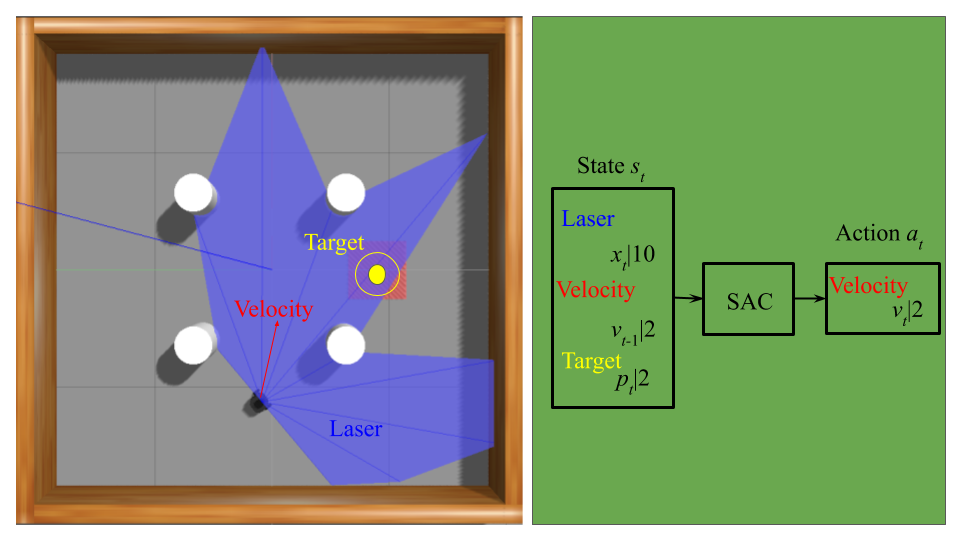
\includegraphics[width=\columnwidth]{images/mapless.png}}
\caption{System definition.}
\label{fig:mapless}
\end{figure}

This work is divided in seven sections.
After a brief introduction in the first section of the Deep-RL on the mobile robot navigation, the second section describes the work of authors on the field that inspired this research, the third section gives a background about the used technique, the fourth section makes an introduction of the tools used for the project, the fifth section summarizes the methods so that the robot can get to a target, the sixth section presents the results obtained on the Gazebo environments, the seventh section makes the discussion on the results and applications of Deep-RL.

\section{Related Works}

Deep-RL has been previously applied on robotic tasks, among these applications we can refer to the work of \cite{kober2013reinforcement}, \cite{stone2005reinforcement}, \cite{tobin2017domain}.
Which is a survey of different works of these techniques applied to robotics.
Mnih et al. \cite{mnih2013playing} utilized a convolution neural network to estimate a value function for future rewards on the Atari games, this strategy was called deep Q-network (DQN) \cite{mnih2013playing}, \cite{hausknecht2015deep}, \cite{van2016deep}.
The DQN can only be used in a task with a discrete action.
To extend it to a continuous control, Lillicrap et al. \cite{lillicrap2015continuous} proposed a deep deterministic policy gradients (DDPG).
That became the basement for the application of Deep-RL in mobile robot navigation as well as the creation of new techniques like the soft actor-critic (SAC) \cite{haarnoja2018soft}.
Tai et al. \cite{tai2017virtual} created a mapless motion planner for a mobile robot by taking the sparse 10-dimensional range findings and the target position with respect to the mobile robot coordinate frame as inputs and the continuous steering commands as output, but firstly being proposed as discrete steering commands on \cite{tai2016towards}. It was shown that, with the asynchronous Deep-RL method, a mapless motion planner can be trained and complete the task to get to a determined target. 

Zhu et al. \cite{zhu2017target} proposed another model to apply the Deep-RL to the task of driving a mobile robot.
The model created took the current observation of states and the image of the target as input and generated an action in a 3D environment as the output.

An activity that can be very challenging in robotics is to navigate a vehicle safely and efficiently in pedestrian-rich environments. Chen et al. \cite{chen2017socially} elaborated a Deep-RL model that can quantify what \textit{to} do and \textit{not to} do on the precise mechanism of human  navigation.
This work develops a time-efficient navigation policy that respects common social norms.
Creating a method able to control a mobile robot moving at human walking speed in an environment with many pedestrians.

\section{Theoretical Background}

The goal in deep reinforcement learning is to control an agent attempting to maximize a reward function. 
The deep Q-network (DQN) algorithm \cite{mnih2013playing} was capable of human level performance on many Atari video games by estimating the actions of an agent.
However, while DQN could solve problems on complex observation spaces, it only can handle discrete action spaces. 
It is noticeable that many tasks, on the robotic control, have continuous action spaces. 
So DQN cannot be applied to continuous domains and it is necessary to use another algorithm that can handle this type of problems.

\subsection{Soft Actor Critic}

The Soft Actor Critic (SAC) algorithm consists of an stochastic actor-critic method that uses approximation functions that can learn continuous action space policies \cite{haarnoja2018soft}. 
The algorithm makes use of a neural network for the actor network, the value network and other for the critic network. 
These three networks computes the action prediction for the current state and generates a temporal-difference error signal for each time step.

% The input of the actor network is the current state, and the output is a real value representing an action chosen for a continuous action space. 
% The output of the critic is simply the estimated Q-value of the current state and the action given by the actor.

Instead of only seeking to maximize the rewards of the system, SAC seeks to also maximize the entropy of the policy.
The entropy refers to how unpredictable a variable can be. 
So, if a random variable always takes a single value then it has zero entropy because it is not unpredictable at all. 
The high entropy in the policy explicitly encourages exploration of the agent because it assigns equal probability to actions that have the same or nearly equal Q-value and also to ensure that it does not collapse into repeatedly selecting a particular action that could exploit some inconsistency in the approximated Q function.


\section{Experimental Setup}

For the analysis of a SAC network was used the programming language Python \cite{ascher1999learning}. 
The Python language has as priority the legibility of the code under speed. 
The vast libraries and frameworks provided by Python makes it an exquisite tool for machine learning and data analysis purposes.

\subsection{ROS}

The robot operations system (ROS) is a flexible framework to write software for robots.
ROS \cite{pyo2015ros} is a collection of tools, and libraries.
ROS provides operational system standard services, like hardware's abstraction, device low level control, messages between processes and package management. 
The set of ROS processes in execution are represented by graphs architecture where the processing is performed on nodes that receive and send messages as sensors, control, state, planning, actuator and others.

Despite the importance of low latency on the robots control, ROS is not a real-time operational system, although it is possible to integrate ROS with real-time code. This lack of real-time system is being addressed on the development of ROS 2.0.

\subsection{Gazebo}

Robot simulation is an essential tool on all roboticist's toolbox.
A good simulator makes possible to test algorithms quickly, to design robots, and to train systems with artificial intelligence using realistic scenarios.
With Gazebo \cite{fairchild2016ros} is possible to simulate this environments easily and with the advantage of having an active community.
This makes Gazebo a great tool on the area of robotic simulation.

\subsection{Turtlebot}

Turtlebot is a ROS standard platform robot, and there are 3 version of the series. Turtlebots are affordable and programmable mobile robots for use in education, research, hobby, and product prototyping.
The third version was used on this project and it is shown in Fig. \ref{fig:turtlebot3}.

\begin{figure}[htbp]
\centerline{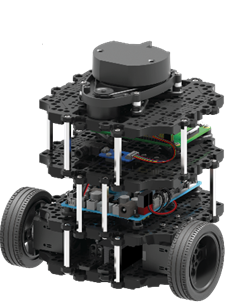
\includegraphics[width=4cm]{images/burger_real.png}}
\caption{Real Turtlebot3 version Burger.}
\label{fig:turtlebot3}
\end{figure}

The Turtlebot3 Burger uses 2 DYNAMIXEL motors series XL, for the object detection the Turtlebot3 utilize a 360 degree sensor laser LiDAR, and it has an IMU sensor for the odometry calculations.
All the control is made by the open source controller board OpenCR1.0 and Raspberry Pi 3 microprocessor.
% The Table \ref{tab1} shows all hardware specification of the Turtlebot3 version Burger.


% \begin{table}[htbp]
% \caption{Hardware Specification of the Turtlebot3 Burger}
% \begin{center}
% \begin{tabular}{|l|l|}
% \hline
% \textbf{Items}&\textbf{Specification} \\
% \hline
% Maximum translational velocity & 0.22 m/s \\
% \hline
% Maximum rotational velocity    & 2.84 rad/s (162.72 deg/s) \\
% \hline
% Maximum payload                & 15kg \\ 
% \hline
% Size (L x W x H)               & 138mm x 178mm x 192mm \\
% \hline
% Weight                         & 1kg \\
% \hline
% Threshold of climbing          & 10 mm or lower \\
% \hline
% Expected operating time        & 2h 30m \\
% \hline
% Expected charging time         & 2h 30m \\
% \hline
% SBC (Single Board Computers)   & Raspberry Pi 3 Model B and B+ \\
% \hline
% Actuator                       & DYNAMIXEL XL430-W250 \\
% \hline
% LDS(Laser Distance Sensor)     & 360 Laser Distance Sensor LDS-01 \\
% \hline
% IMU                            & \begin{tabular}[c]{@{}c@{}}Gyroscope 3 Axis\\ Accelerometer 3 Axis\\ Magnetometer 3 Axis\end{tabular} \\
% \hline
% Battery                        & \begin{tabular}[c]{@{}c@{}}Lithium polymer \\ 11.1V 1800mAh / 19.98Wh 5C \\ \end{tabular} \\
% \hline

% \end{tabular}
% \label{tab1}
% \end{center}
% \end{table}

% \subsection{OpenCV}

% Open Source Computer Vision (OpenCV) is an open source computer vision and machine learning software library.
% It is mainly used for developing advanced image processing and computer vision applications \cite{bradski2008learning}, \cite{wang2010camera}.
% OpenCV can take frames out of a video and run algorithms to get necessary information.
% It can also identify an object, recognize a face or track the movement of an object.
% It is commonly used in robotics \cite{oyama2009come}.

\subsection{Simulation Environments}

There were used two environments for the simulations. The first environment is  shown in Fig. \ref{subfig:env1}, the environment represents a free area for the robot to move.
The walls of this environment are the only things where the robot can collide.
If the mobile robot collide with the wall or any obstacle, a negative reward is given for this action and the current episode stops.
The second environment is shown in Fig. \ref{subfig:env2} and has 4 fixed obstacles.
It means that this environment is more complex in a way that the intelligent agent have to make a better strategy to not collide.
% The third environment, shown in {\color{blue}Figure} \ref{fig:environments}{\color{blue}(c)}, is more complex than the previous environments.  
% The number of walls and the mobile obstacles, represented by the white blocks, makes the environment more dynamical, approaching it to a real-world scenarios.



\begin{figure}[htbp]
    \centering
    \begin{subfigure}[b]{0.2\textwidth}
        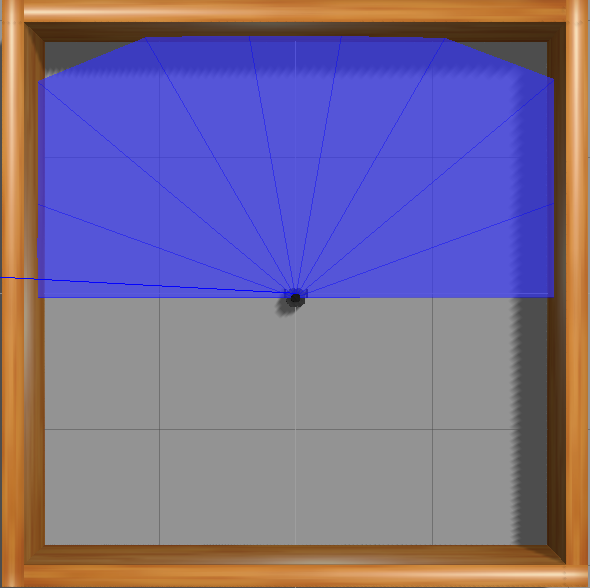
\includegraphics[width=\textwidth]{images/amb1.png}
        \caption{First environment.}
        \label{subfig:env1}
    \end{subfigure}
    ~ %add desired spacing between images, e. g. ~, \quad, \qquad, \hfill etc. 
      %(or a blank line to force the subfigure onto a new line)
    \begin{subfigure}[b]{0.2\textwidth}
        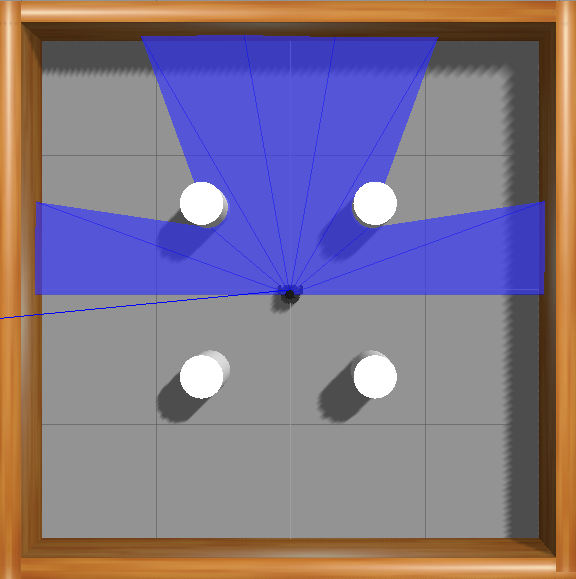
\includegraphics[width=\textwidth]{images/amb2.png}
        \caption{Second environment.}
        \label{subfig:env2}
    \end{subfigure}
    \caption{Training environments used on Gazebo simulation.}\label{fig:environments}
\end{figure}

% \begin{figure}[H]
% \centerline{\includegraphics[width=\columnwidth]{images/environments1.png}}
% \caption{Training environments used on Gazebo simulation. First environment (a), second environment (b) and third environment (c).}
% \label{fig:environments}
% \end{figure}

\subsection{Real Environments}

After training the SAC network through simulation, it will be tested in a real scenario.
The Turtlebot3, version Burger, will be used to perform this test.
Some of the necessary inputs of the network in the real environment were obtained by image processing.
The first real environment is shown in Fig. \ref{subfig:real_env1} and resembles the first simulation with no obstacles. The second environment is shown in Fig. \ref{subfig:real_env2} and it presents a complex environment similar to the second used on simulation.

\begin{figure}[htbp]
    \centering
    \begin{subfigure}[t]{0.22\textwidth}
        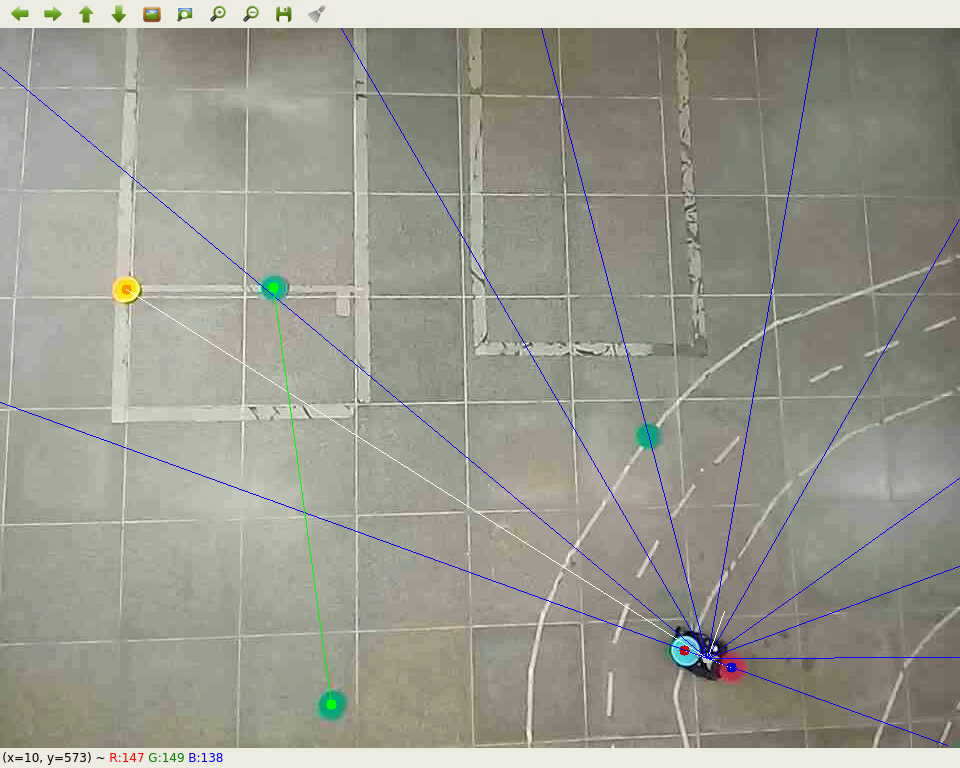
\includegraphics[width=\textwidth]{images/test_env1/1.png}
        \caption{First real environment.}
        \label{subfig:real_env1}
    \end{subfigure}
    ~
    \begin{subfigure}[t]{0.22\textwidth}
        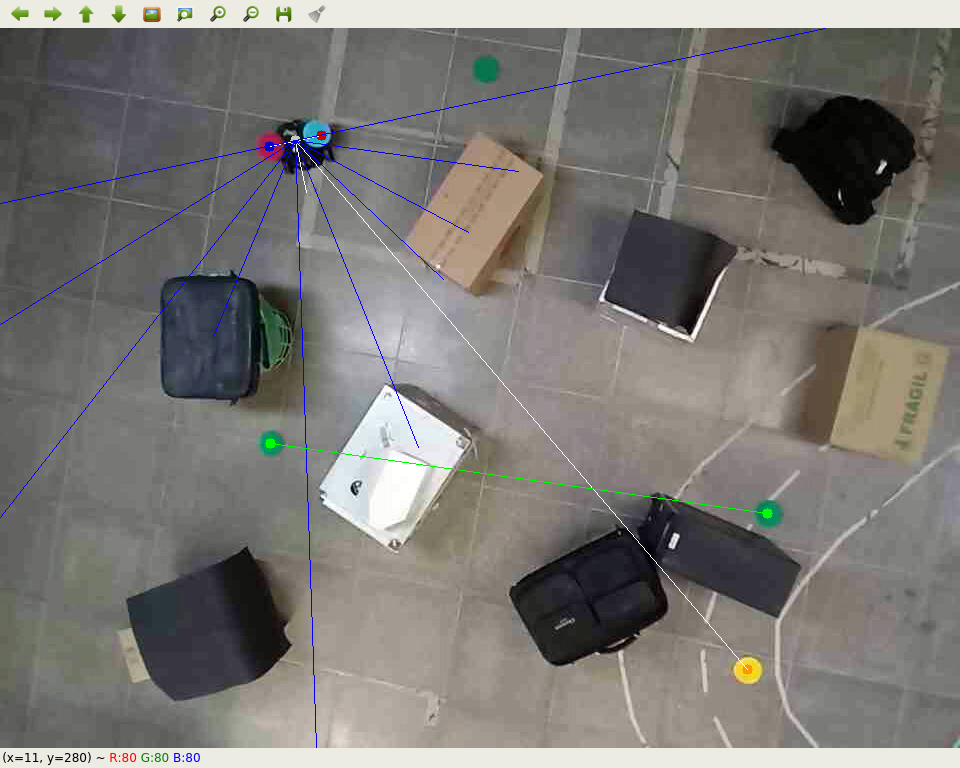
\includegraphics[width=\textwidth]{images/test_env2/1.png}
        \caption{Second real environment.}
        \label{subfig:real_env2}
    \end{subfigure}
    \caption{Environments created for the SAC test on the real world.}\label{fig:real_environments}
\end{figure}

\section{Methodology}

The intention of this work is to propose a system for a mobile robot in order to plan its movements without any map knowledge on the environment. Its translation function is defined as:
\begin{equation}
v_t = f(x_t, p_t, v_{t-1})
\end{equation}
where $x_t$ is the observation from the raw sensor information, $p_t$ is the relative position of the target, and $v_{t-1}$ is the velocity of the mobile robot in the last time step.
All variables specified, previously, can be defined as the current state $s_t$ of the mobile robot.
With this model it is possible to get the actions that the robot will make, given its current state.
However, it is needed to ensure a minimum reading frequency of the input data to control the movement of the robot because if the robot get a slow read frequency of the inputs it cannot react to an obstacle in the trajectory to a target. In this way, the robot can react to new states quickly.
This method was first explored by Tai et al. \cite{tai2017virtual}.

\subsection{Network Structure}

Once the system of state and actions has been defined, it is possible to create a SAC network capable of resolving the problem.
The SAC network has 14 inputs as presented in Fig. \ref{fig:entradaESaida}, in which 10 corresponds to the laser range findings, 2 corresponds to the previous linear and angular velocity, and the other 2 corresponds to the relative position and angle of the mobile robot to the target.
The sample of the laser range findings are between $-90$ and $90$ degrees in relation to the robot. The output of the network is the action of linear and angular velocity that will be applied on the mobile robot.

\begin{figure}[htbp]
\centerline{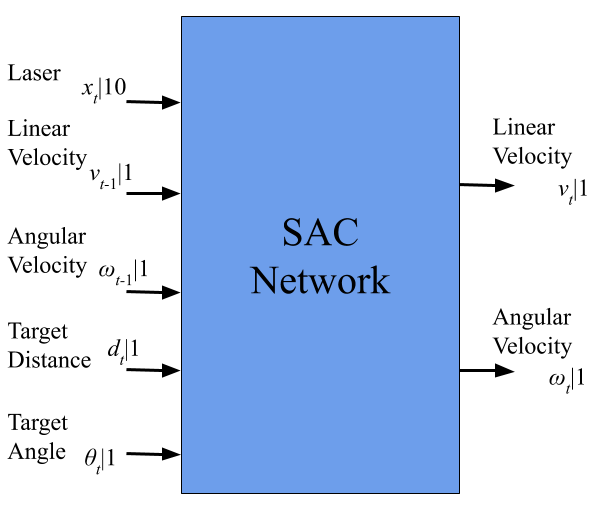
\includegraphics[width=\columnwidth]{images/output_and_input.png}}
\caption{SAC network inputs and outputs.}
\label{fig:entradaESaida}
\end{figure}

The network structure of the SAC is shown in Fig \ref{fig:projetointegrador}. 
The actor-network has as input the current state of the mobile robot followed by 4 fully-connected neural networks layers with 512 nodes.
This input of the networks is transformed on the linear and angular velocity that will be the commands sent to the motor of the mobile robot. 
The action range is constrained between $(-1,1)$ and the hyperbolic tangent function $(tanh)$ is used as activation function.
The outputs of the action are then changed for the linear velocity that varies between $0$ to $0.22$ $m/s$ and the angular velocity be between $-2$ to $2$ $rad/s$ on the TurtleBot3 robot version Burger.


\begin{figure}[htbp]
\centerline{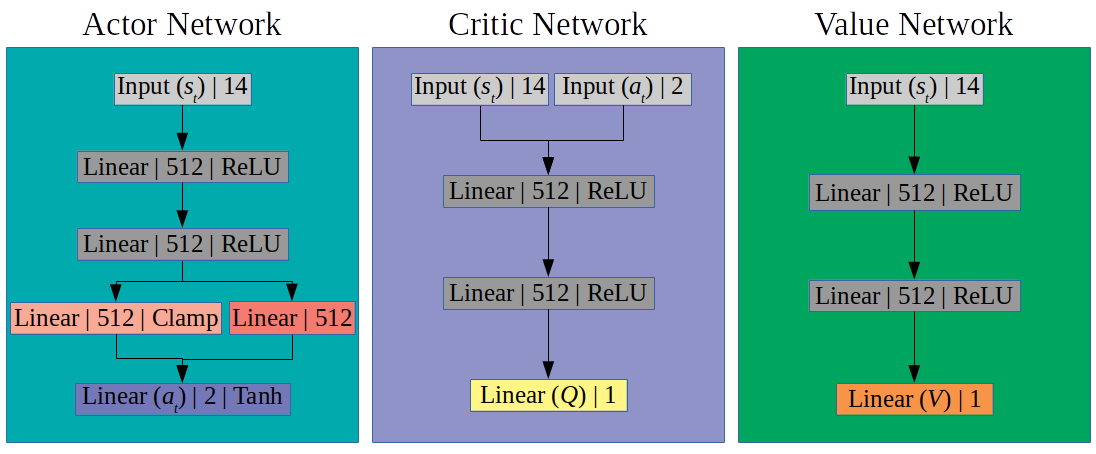
\includegraphics[width=\columnwidth]{images/structure_sac.png}}
\caption{SAC network structure model.}
\label{fig:projetointegrador}
\end{figure}

In the critic-network, the Q-value of the current state and action are predicted.
And in the value-network, the value of the current state is predicted.
The two networks use only 2 fully-connected neural networks layers to process the input state.
The Q-value and the value of the current state is activated through a linear activation function:
\begin{equation}
y = kx +b
\end{equation}
where $x$ is the input of the last layer, $y$ is the predicted Q-value or the predicted value of the current state, and $k$ and $b$ are the trained weights and bias of this layer, respectively.

\subsection{Reward Function}

Once the environment has been defined it is possible to simulate a controlled mobile robot for a navigation task.
It is necessary to define the reward and penalty system to the Deep-RL network.
Remembering that the rewards and penalties are attributed numbers passed to the intelligent agent.
So, the network will make a feedforward and backpropagation step in order to learn the hyperparameters.

There are four different conditions for the reward system that presented better results for the resolution of the problem and are the following:
\begin{equation}
r (s_t, a_t) = 
\begin{cases}
r_{arrive} \ \textrm{if} \ d_t < c_d
\\
r_{collide} \ \textrm{if}\ min_x < c_o
\\
c_{r1}(d_{t-1} - d_t) \ \textrm{if} \ (d_{t-1} - d_t) > 0
\\
c_{r2} \ \textrm{if} \ (d_{t-1} - d_t) \leq 0
\end{cases}
\end{equation}

If the robot gets to the target through threshold checking $c_d$, a positive reward $(r_{arrive})$ is given, but if the robot collides with an obstacle through a minimum range readings checking, a negative reward $(r_{collide})$ is given.
Both conditions are sufficient to end the training episode.
Otherwise, the reward is based on the distance difference from the target compared to the last time step $(d_{t-1} - d_t)$. 
If this difference is positive the reward given is the distance traveled multiplied by the hyperparameter $(c_{r1})$, and if the distance is negative is used the hyperparameter $(c_{r2})$.
This motivates the mobile robot to get closer to the target position and encourages it to avoid the obstacles in the environment.

% \subsection{Positioning capture in real environments}

% After training the SAC network through simulation, it will be tested in a real scenario.
% The Turtlebot3, version Burger, will be used to perform this test.
% It will be necessary to obtain the angle and distance of a target for the network to complete its goal.
% So it was setup a camera in the ceiling to extract this information.

% Firstly, the essential points positions to extract the angle and distance are taken from the image.
% These positions include the target, left and right side of the robot, and three points to be a distance reference parameter.
% Fig. \ref{fig:pixel_to_meter} shows a frame of the scenario in which there were used different colored circles to identify the relevant points.
% The yellow circle was attached as the target, the blue to the left side of the robot, the red to the right side and the three green circles were used as reference parameter to calculate the distance.

% \begin{figure}[htbp]
% \centerline{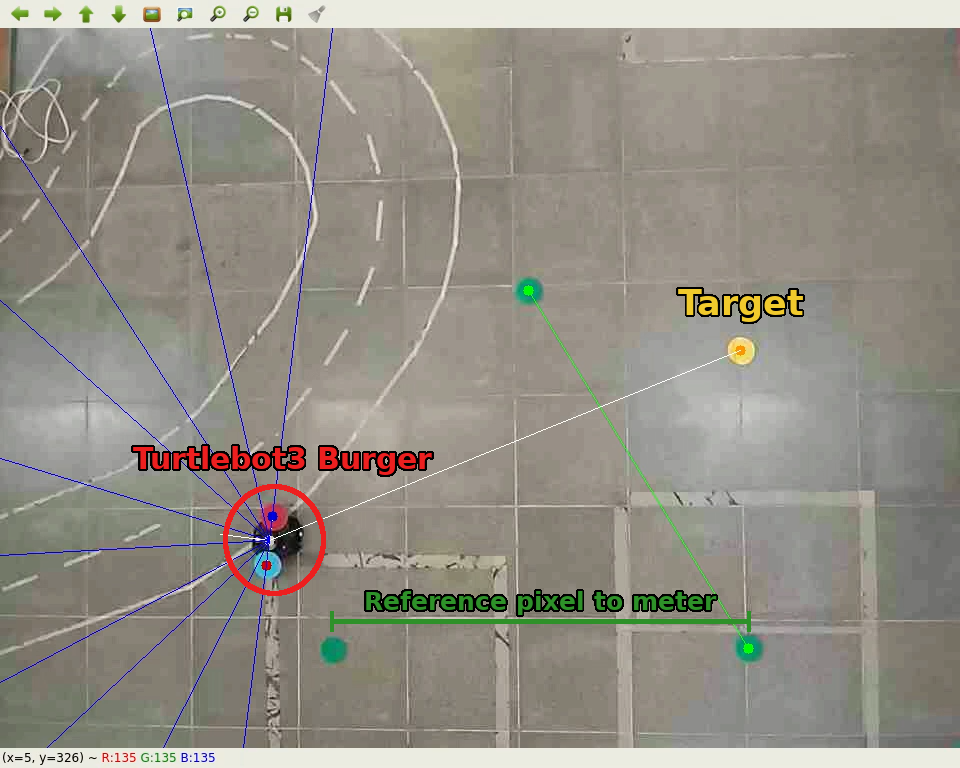
\includegraphics[width=6cm]{images/pixel_to_meter.png}}
% \caption{Real environment relevant points}
% \label{fig:pixel_to_meter}
% \end{figure}


% After the points were extracted from the center of the circles, it is possible to calculate the two necessary SAC network inputs.
% So, it is necessary to figure out the vector distance that connects the center of the Turtlebot3 to the target point, and the vector direction which represents the direction of the robot.
% The distance and angle between the mobile robot and the target are calculated frame by frame, and it is used as the necessary inputs of the SAC network simultaneously.



%aqui vou escrever mais 
%The center of green circles have a predefined distance from each other, what permits the calculation of robot and target distance by converting the pixel distance of the image to the distance in meters.
%aqui tbm





%After the points were extracted from the center of the circles, it is possible to calculate the two necessary SAC network inputs.
%So, it is necessary to figure out the vector $distance$ that connects the center of Turtlebot3 to the target point, and the vector $direction$ which represents the direction of robot.
%The vector $direction$ starts from the center of Turtlebot3, which is equal to the midpoint of the blue and red points.
%The blue and red circles are on left and right sides of the mobile robot, respectively.
%With this it is possible to determine the front of the robot.

%aqui vou escrever mais 
%The center of green circles have a predefined distance from each other, what permits the calculation of robot and target distance by converting the pixel distance of the image to the distance in meters.
%aqui tbm



% e aeee
%acabei de perder meia hora no face AAAAAAA
% cara, na escrita n me dou mt bem, mas vou escrevendo o q vem na cabeça e após a gente estrutura melhor
% faz isso mesmo meu KKKK eu sou meio travado na vdd mas to tentando (bem travado)
% a ideia é meter o louco e escrever tudo que vem na mente
% isso vem com a pratica SAUHSUAS, 
% pode se sentir a vontade pra mudar as coisas.
% só modifiquei pq achei melhor - ficou melhor assim msm ;)
% o que tu conseguir escrever eu e o professor gamarra corrigimos depois


%qual tu pensa a imagem pra colocar nessa subsection ae
%um frame com o alvo indicado, pixel meter parameter tb, e o robo? q nem o video do face? ---> meu acho que pode ser só uma imagem que contenha o robo, a referencia e tals (pode ser do primeiro ambiente que a gente tinha feito) ai tu explica através dela - OK

%coloquei a imagem do grafico com os obstáculos no drive, acho q ficou ok ---> eu vi, tá top na real - :D
% amanhã vou pegar pra escrever nos resultados, tava editando o modelo mais hj - azulzinho topi --> e as imagens pra ficarem melhor tbm
% vou pegar pra dormir aqui na real, flws o/// falooooow veéeei até amanhã


\section{Results}

This section deals with the presentation and discussion of results.
The collected data are related to the obtained reward from the artificial neural network of the project.
With these data is possible to see what is the learning degree of the agent in the environment because the gained reward is intrinsically attached to the performance of the agent on the environment that it must go.
All the training environments were arranged by ROBOTIS, however, some alterations were done on the source code of the Gazebo simulation in order to use the simulated mobile robot and the reward function defined on this paper.

\subsection{Simulation Results}

A mobile robot with a SAC network was trained in order to make the experiments in the environments presented on Fig. \ref{fig:environments}, where the goal of the mobile robot is to get to the target.
The initial test used the first environment defined. It is shown in Fig. \ref{fig:frames_simenv1} a sequence of frames of the robot and the target. 
We can observe how the robot starts in an initial position distant from the target, navigating in order to reach the target.

\begin{figure}[htbp]
    \centering
    \begin{subfigure}[b]{0.115\textwidth}
        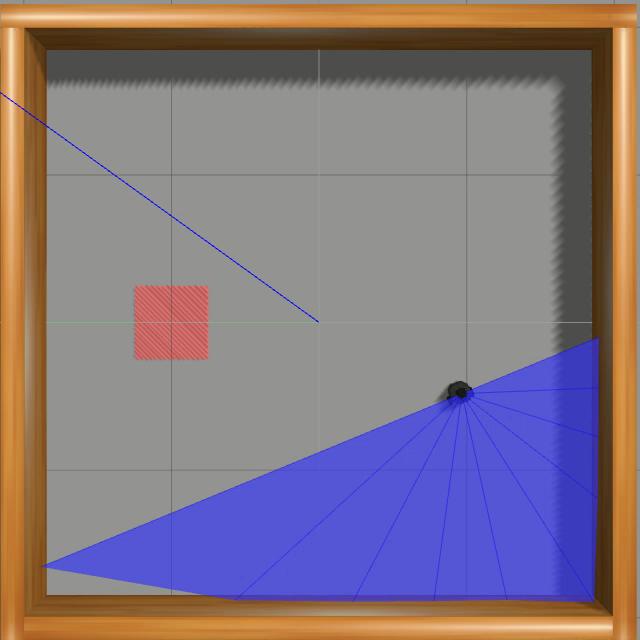
\includegraphics[width=\textwidth]{images/simenv1/1.png}
    \end{subfigure}
    \hfill
    \begin{subfigure}[b]{0.115\textwidth}
        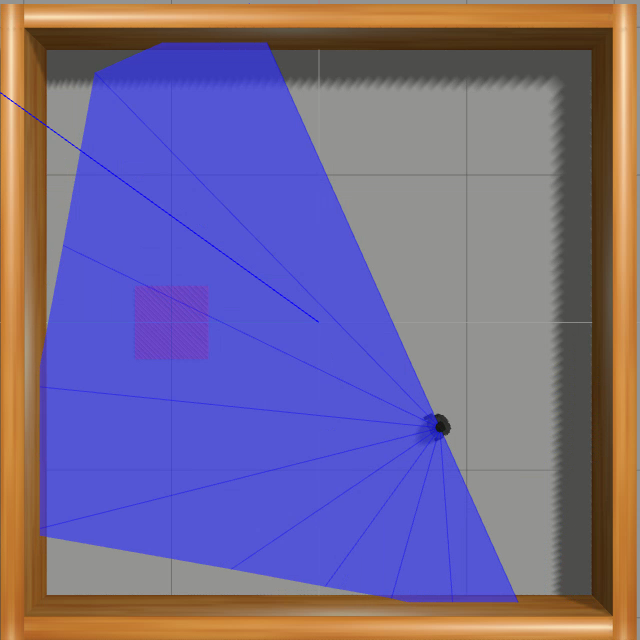
\includegraphics[width=\textwidth]{images/simenv1/2.png}
    \end{subfigure}
    \hfill
    \begin{subfigure}[b]{0.115\textwidth}
        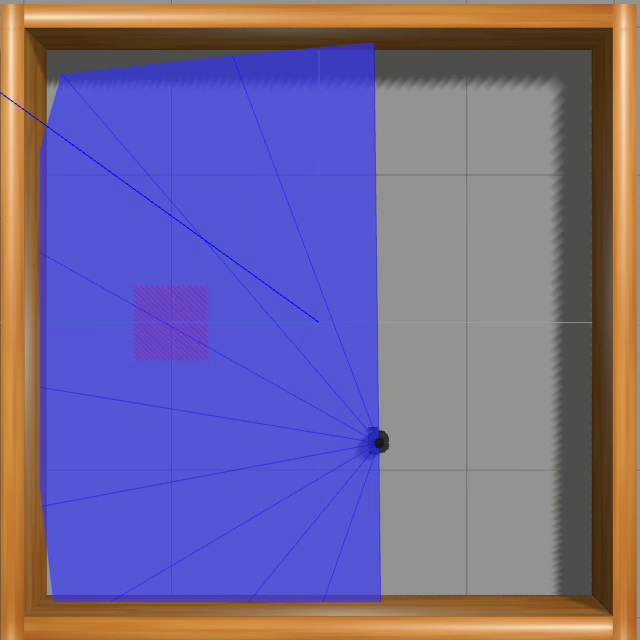
\includegraphics[width=\textwidth]{images/simenv1/3.png}
    \end{subfigure}
    \hfill
    \begin{subfigure}[b]{0.115\textwidth}
        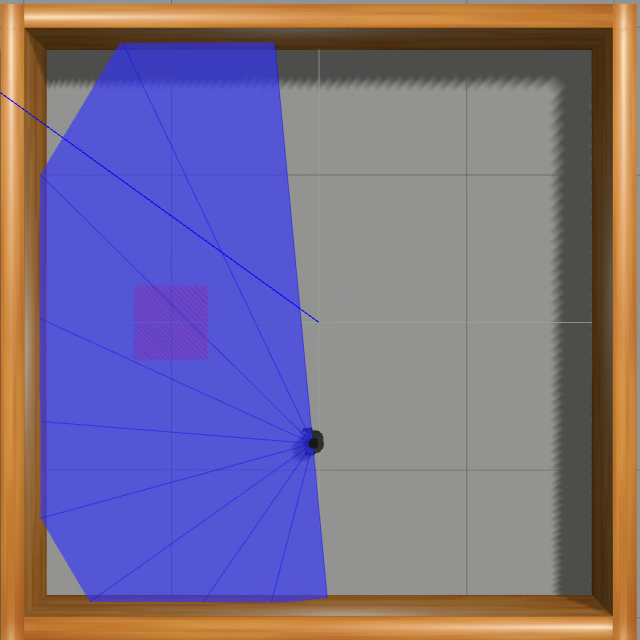
\includegraphics[width=\textwidth]{images/simenv1/4.png}
    \end{subfigure}
    \newline
    \begin{subfigure}[b]{0.115\textwidth}
        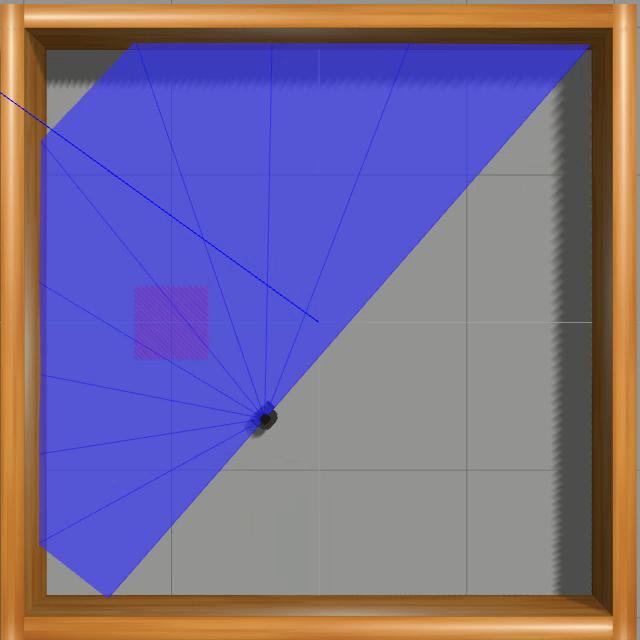
\includegraphics[width=\textwidth]{images/simenv1/5.png}
    \end{subfigure}
    \hfill
    \begin{subfigure}[b]{0.115\textwidth}
        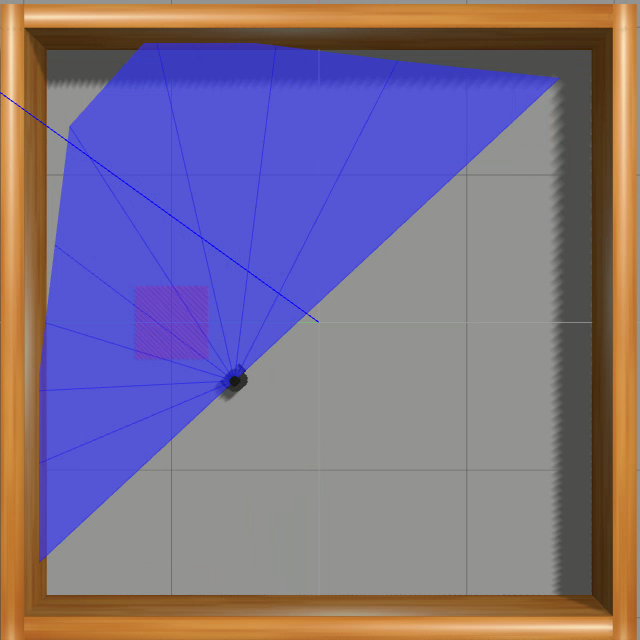
\includegraphics[width=\textwidth]{images/simenv1/6.png}
    \end{subfigure}
    \hfill
    \begin{subfigure}[b]{0.115\textwidth}
        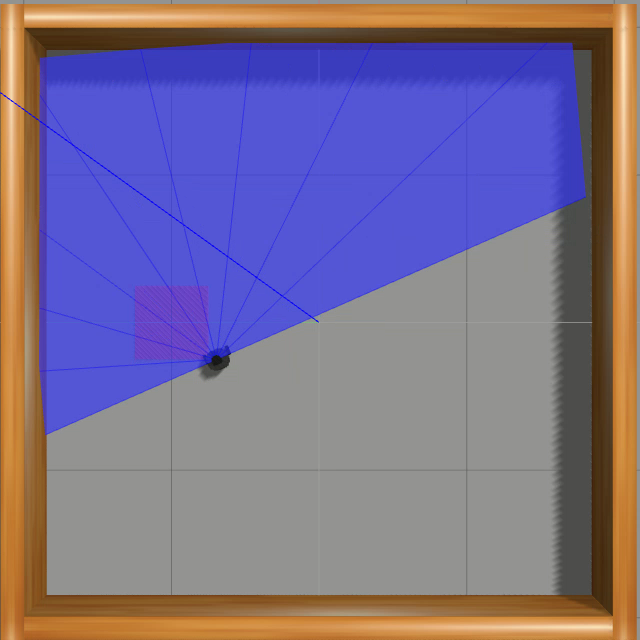
\includegraphics[width=\textwidth]{images/simenv1/7.png}
    \end{subfigure}
    \hfill
    \begin{subfigure}[b]{0.115\textwidth}
        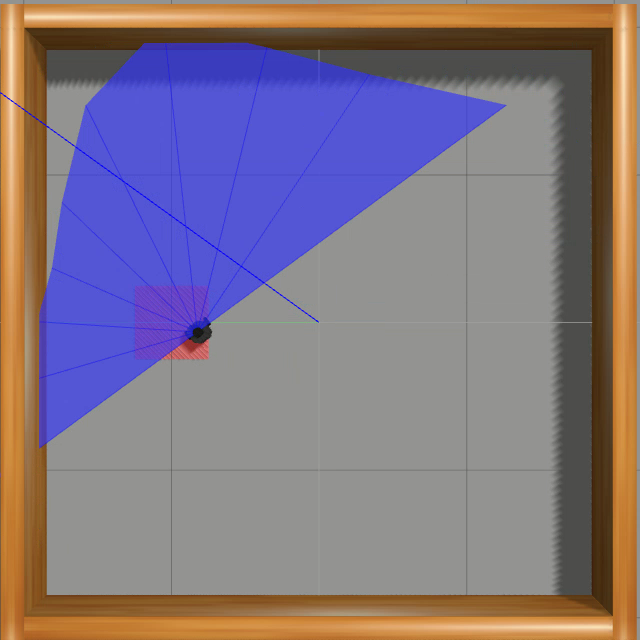
\includegraphics[width=\textwidth]{images/simenv1/8.png}
    \end{subfigure}
    \caption{Images sequence in the first simulated environment of the experiment.}\label{fig:frames_simenv1}
\end{figure}


The training results of the reward function of the first environment are shown in Fig. \ref{fig:stage_1}.
On the first episodes can be noticed a negative reward, this happens because the algorithm started and it was still learning.
This reward by episode means that the robot is trying to maximize the reward to complete the task.

\begin{figure}[htbp]
\centerline{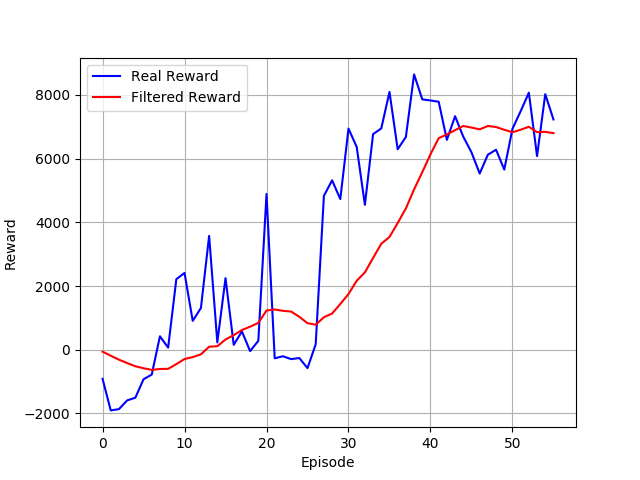
\includegraphics[width=\columnwidth]{images/stage_1.png}}
\caption{Rewards of the first environment.}
\label{fig:stage_1}
\end{figure}

In Fig. \ref{fig:stage_1} the $x$ axis represents the past episodes on the simulation, an episode is defined when the mobile robot arrives to the target in the map or collides with some obstacle. 
The $y$ axis in Fig. \ref{fig:stage_1} represents the total value of the reward that the robot received on the episode.
The reward, with the blue color, has a great variance, it was decided to use a moving average filter for better visualization of the results.

After the mobile robot has been trained on the first environment, the experiment was done in the second environment.
It is shown in Fig. \ref{fig:frames_simenv2} a sequence of the actions made by the Turtlebot from an initial position until it could arrive to the target after the training episodes.

\begin{figure}[htbp]
    \centering
    \begin{subfigure}[b]{0.115\textwidth}
        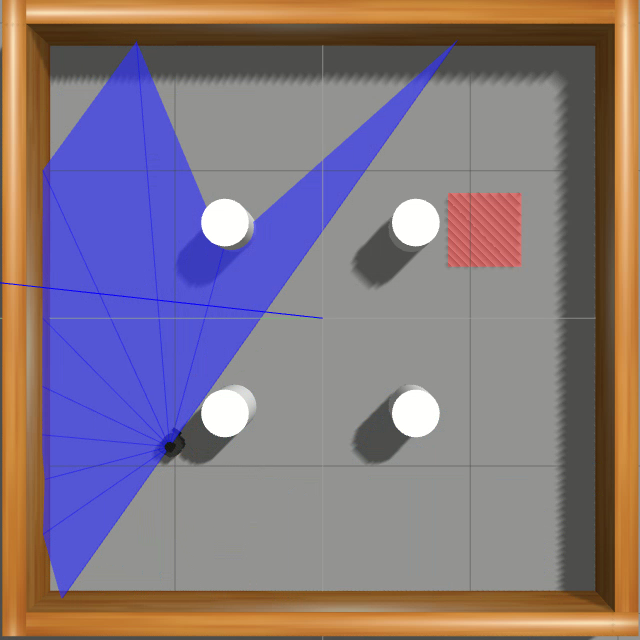
\includegraphics[width=\textwidth]{images/simenv2/1.png}
    \end{subfigure}
    \hfill
    \begin{subfigure}[b]{0.115\textwidth}
        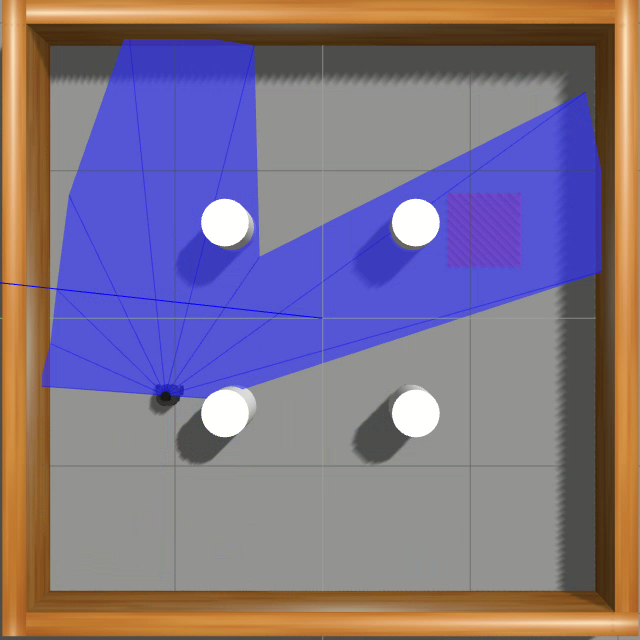
\includegraphics[width=\textwidth]{images/simenv2/2.png}
    \end{subfigure}
    \hfill
    \begin{subfigure}[b]{0.115\textwidth}
        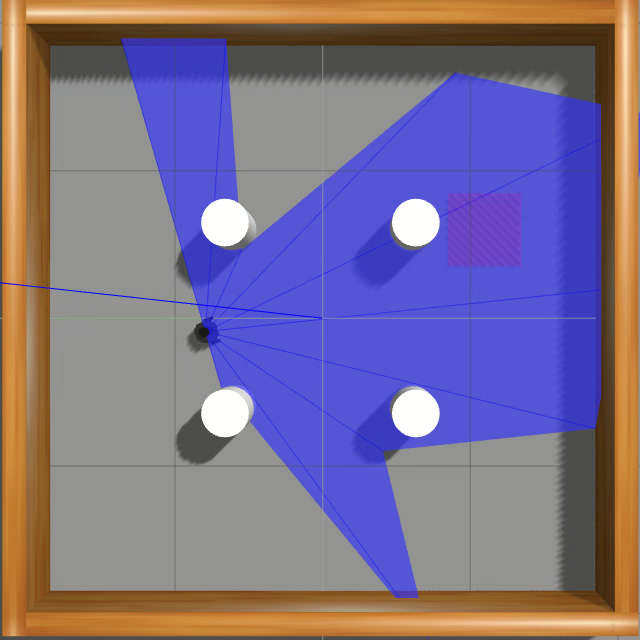
\includegraphics[width=\textwidth]{images/simenv2/3.png}
    \end{subfigure}
    \hfill
    \begin{subfigure}[b]{0.115\textwidth}
        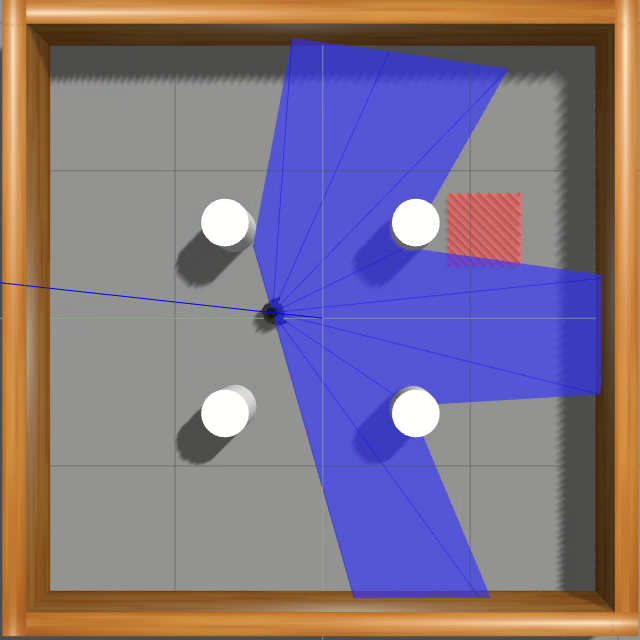
\includegraphics[width=\textwidth]{images/simenv2/4.png}
    \end{subfigure}
    \newline
    \begin{subfigure}[b]{0.115\textwidth}
        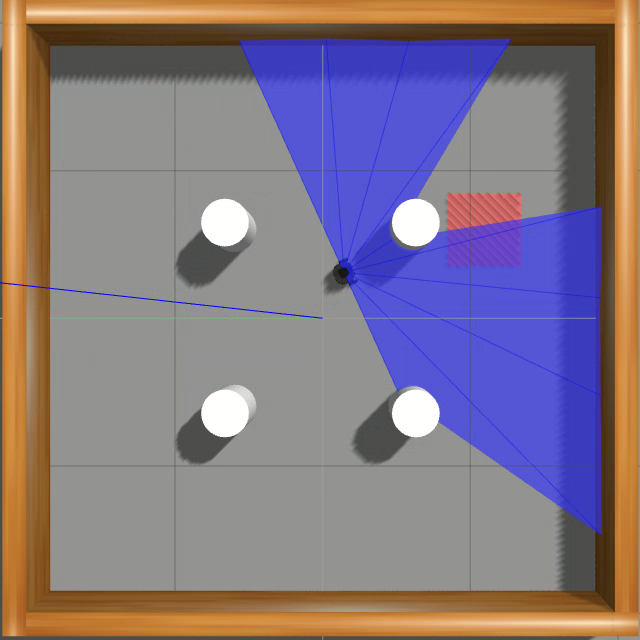
\includegraphics[width=\textwidth]{images/simenv2/5.png}
    \end{subfigure}
    \hfill
    \begin{subfigure}[b]{0.115\textwidth}
        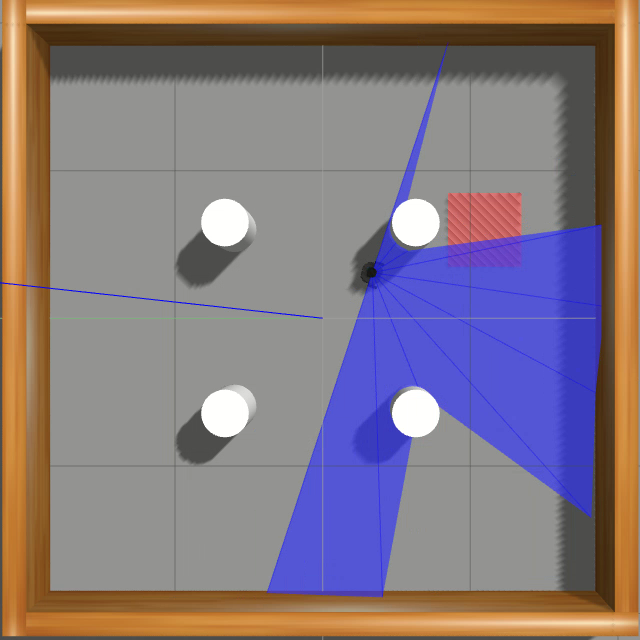
\includegraphics[width=\textwidth]{images/simenv2/6.png}
    \end{subfigure}
    \hfill
    \begin{subfigure}[b]{0.115\textwidth}
        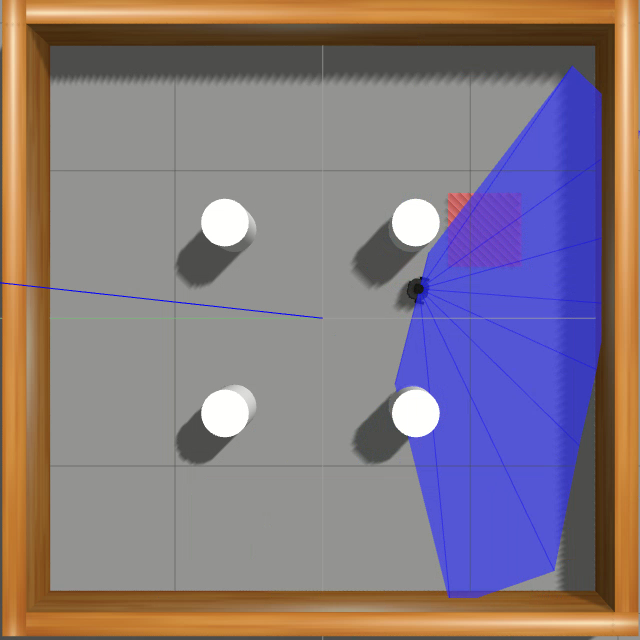
\includegraphics[width=\textwidth]{images/simenv2/7.png}
    \end{subfigure}
    \hfill
    \begin{subfigure}[b]{0.115\textwidth}
        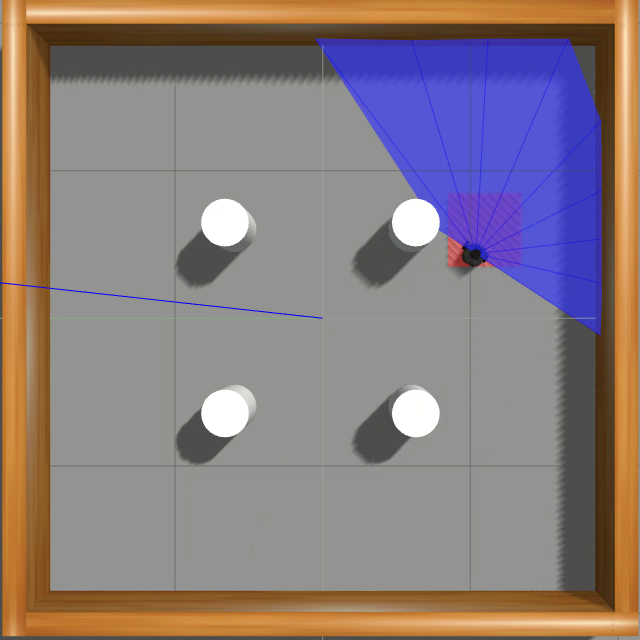
\includegraphics[width=\textwidth]{images/simenv2/8.png}
    \end{subfigure}
    \caption{Images sequence in the second simulated environment of the experiment.}\label{fig:frames_simenv2}
\end{figure}

The reward function results of the training process for the second environment are shown in Fig. \ref{fig:stage_2}.
Comparing this results with the last environment, we can observe that it needed more episodes so the robot could present good results.
It is noticed that with a more complex environment, exists the possibility that an agent could take a longer time to get a good performance.

\begin{figure}[htbp]
\centerline{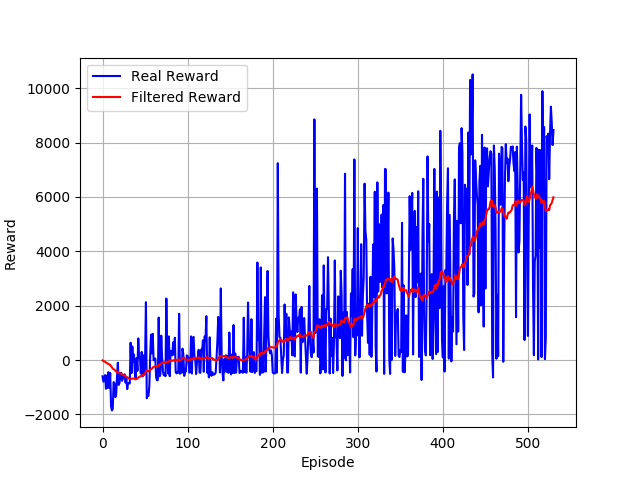
\includegraphics[width=\columnwidth]{images/stage_2.png}}
\caption{Rewards of the second environment.}
\label{fig:stage_2}
\end{figure}

\subsection{Experiments with Turtlebot}

After the training and validation of each simulation environment, there were used the two real environments, presented in the Fig. \ref{fig:real_environments}, for the testing of the SAC network in the real world.
With the target defined on the first real environment, it was executed the SAC network on the Turtlebot3.
In the graph, shown in Fig. \ref{fig:env1_graph}, is possible to see the trajectory made by the network to arrive to the target.
The robot starts at the point $(0, 0)$ and makes a trajectory to get to the target.
Fig. \ref{fig:frames_env1} shows by frames the trajectory made by the robot to complete the task.

\begin{figure}[htbp]
\centerline{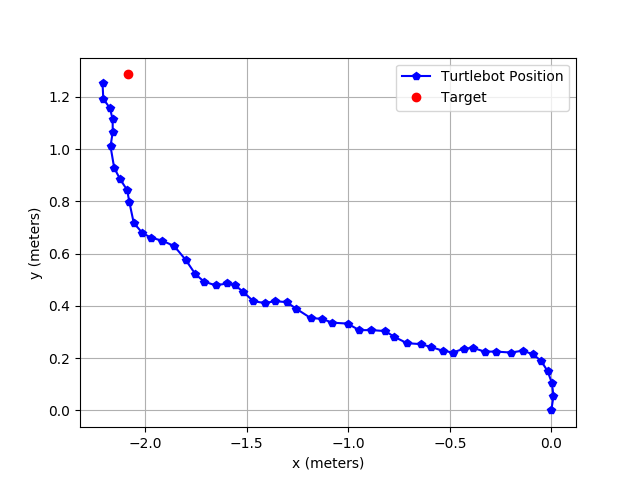
\includegraphics[width=\columnwidth]{images/test_env1.png}}
\caption{Trajectory of the Turtlebot3 in the first real environment}
\label{fig:env1_graph}
\end{figure}

\begin{figure}[htbp]
    \centering
    \begin{subfigure}[b]{0.115\textwidth}
        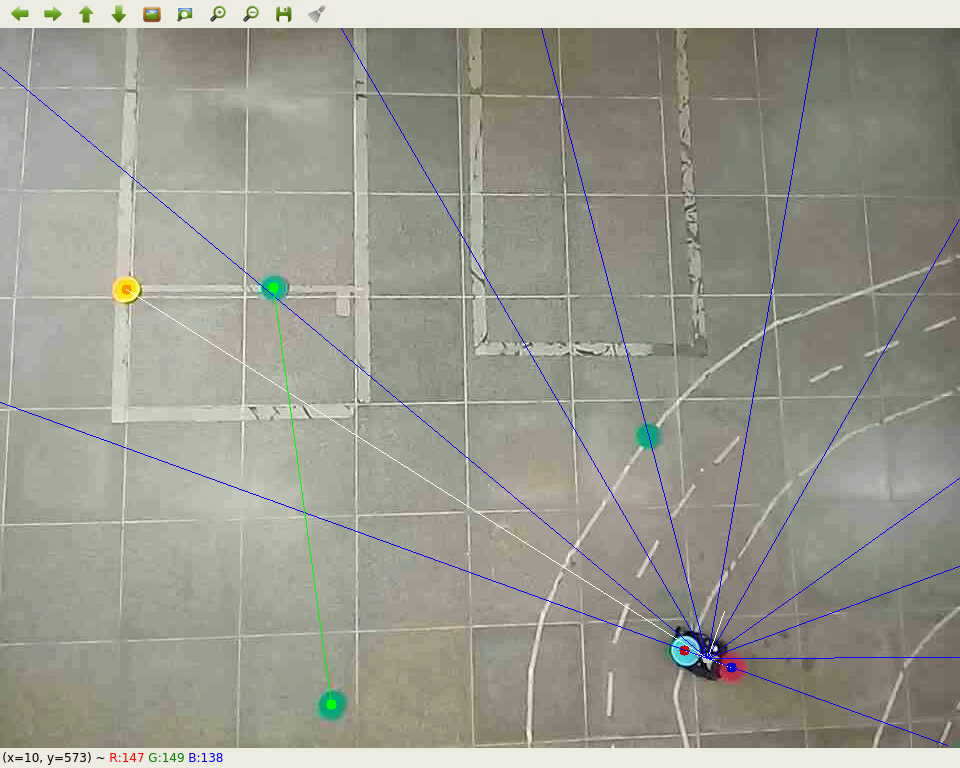
\includegraphics[width=\textwidth]{images/test_env1/1.png}
    \end{subfigure}
    \hfill
    \begin{subfigure}[b]{0.115\textwidth}
        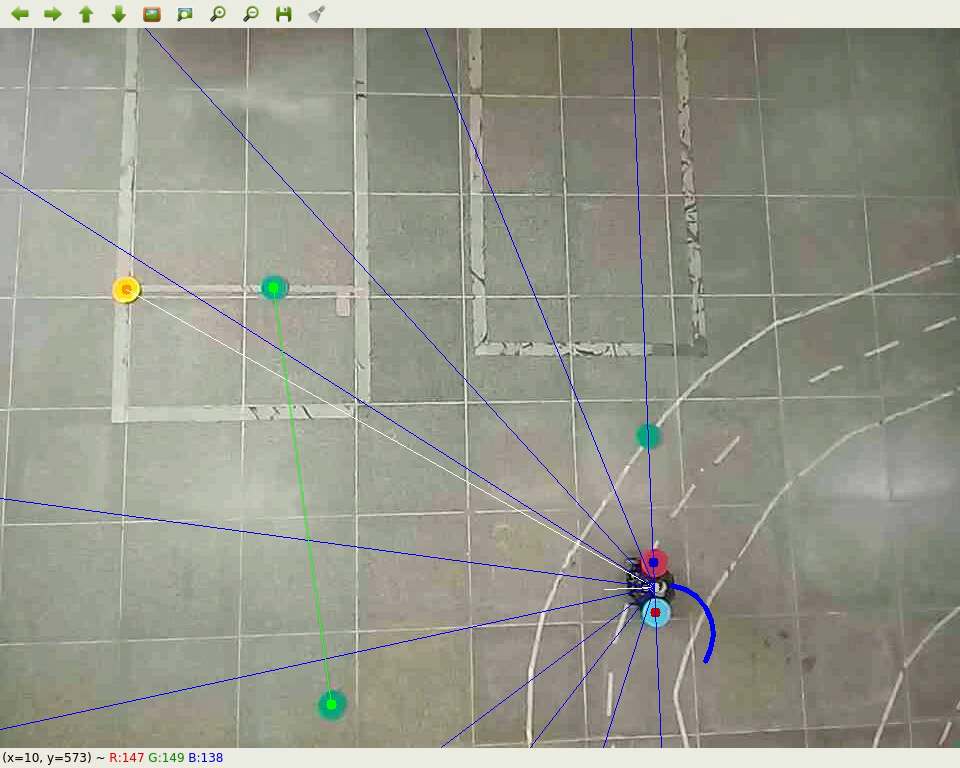
\includegraphics[width=\textwidth]{images/test_env1/2.png}
    \end{subfigure}
    \hfill
    \begin{subfigure}[b]{0.115\textwidth}
        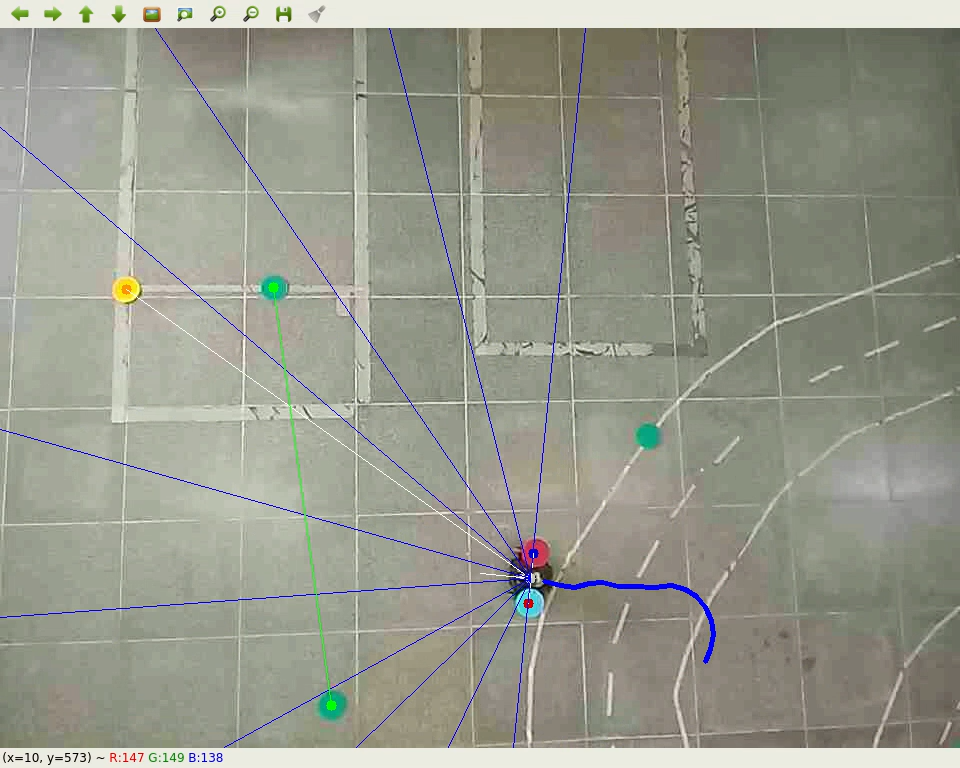
\includegraphics[width=\textwidth]{images/test_env1/3.png}
    \end{subfigure}
    \hfill
    \begin{subfigure}[b]{0.115\textwidth}
        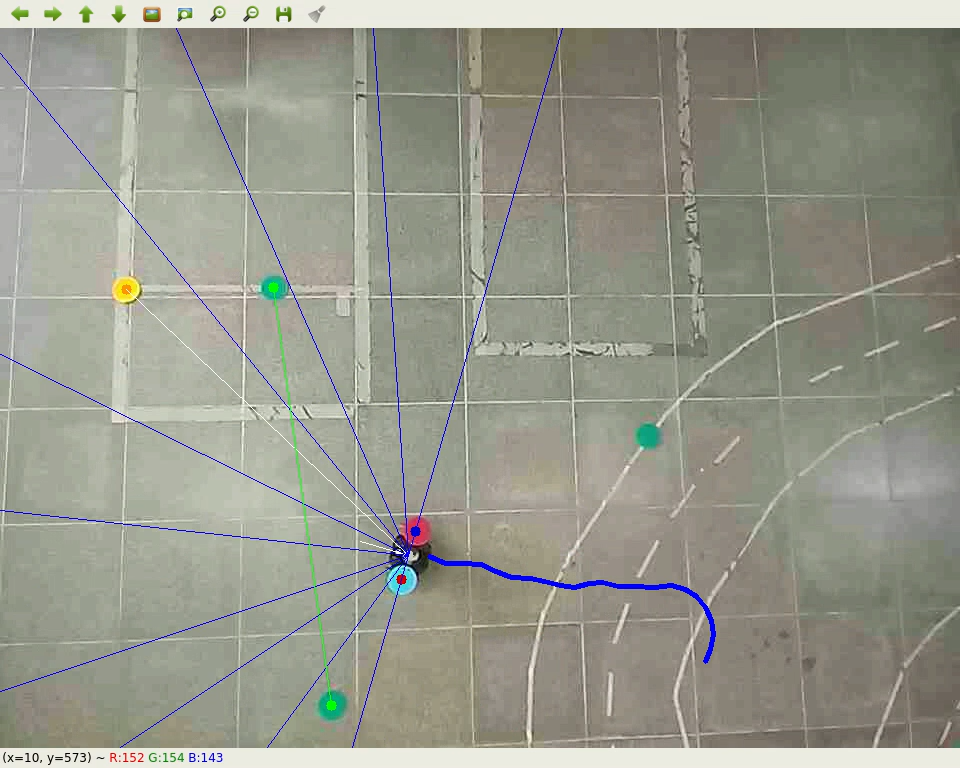
\includegraphics[width=\textwidth]{images/test_env1/4.png}
    \end{subfigure}
    \newline
    \begin{subfigure}[b]{0.115\textwidth}
        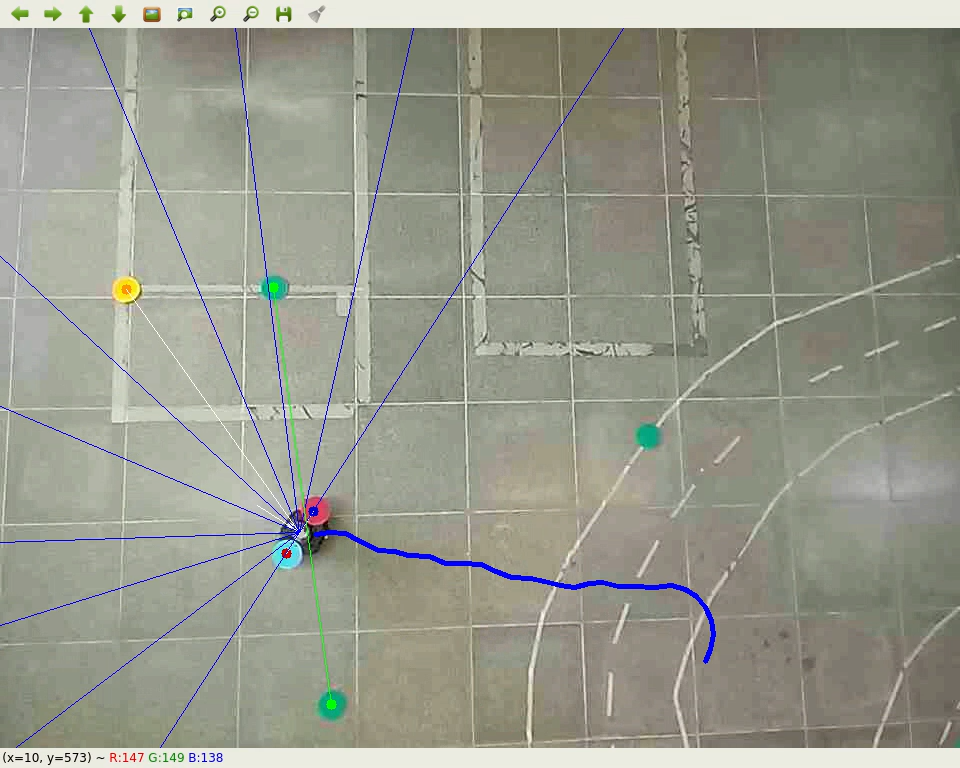
\includegraphics[width=\textwidth]{images/test_env1/5.png}
    \end{subfigure}
    \hfill
    \begin{subfigure}[b]{0.115\textwidth}
        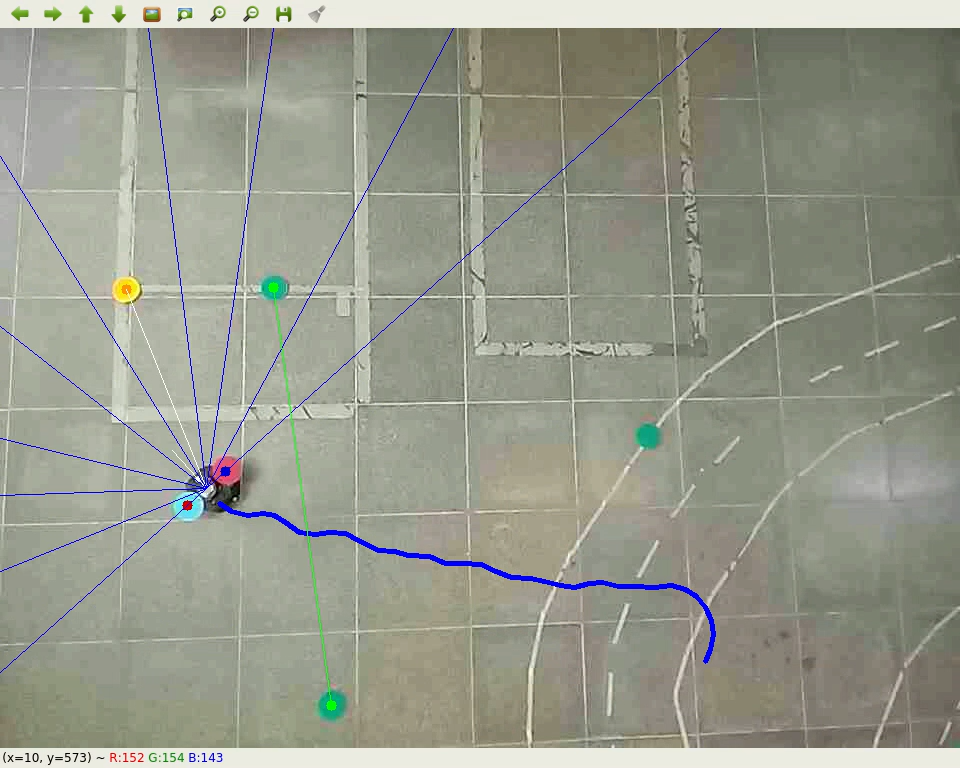
\includegraphics[width=\textwidth]{images/test_env1/6.png}
    \end{subfigure}
    \hfill
    \begin{subfigure}[b]{0.115\textwidth}
        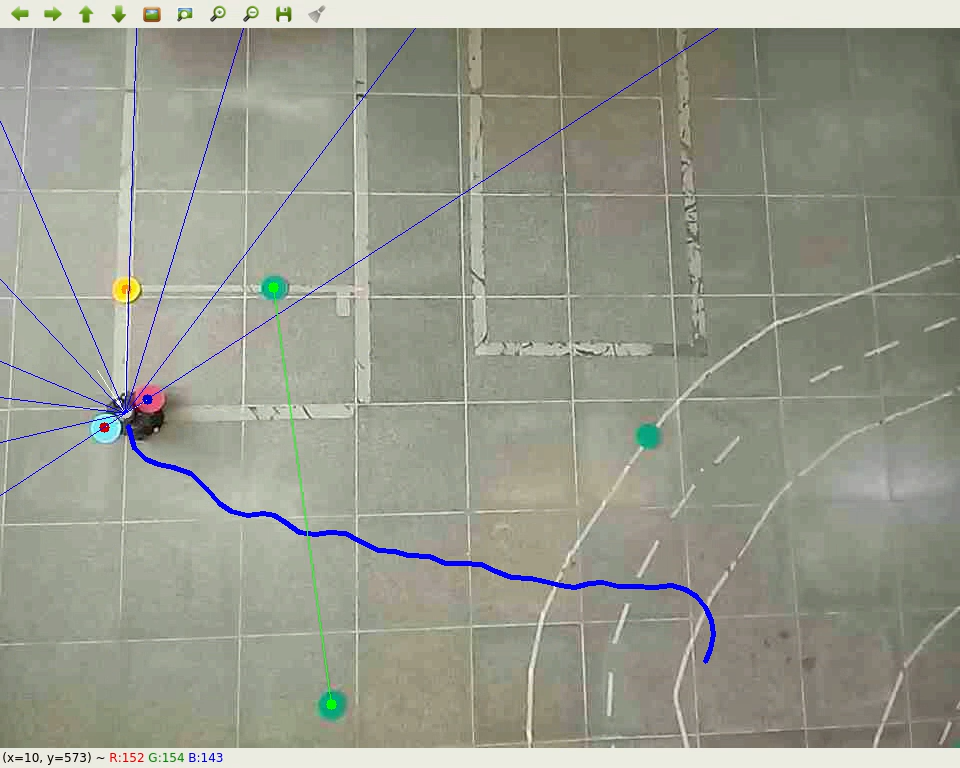
\includegraphics[width=\textwidth]{images/test_env1/7.png}
    \end{subfigure}
    \hfill
    \begin{subfigure}[b]{0.115\textwidth}
        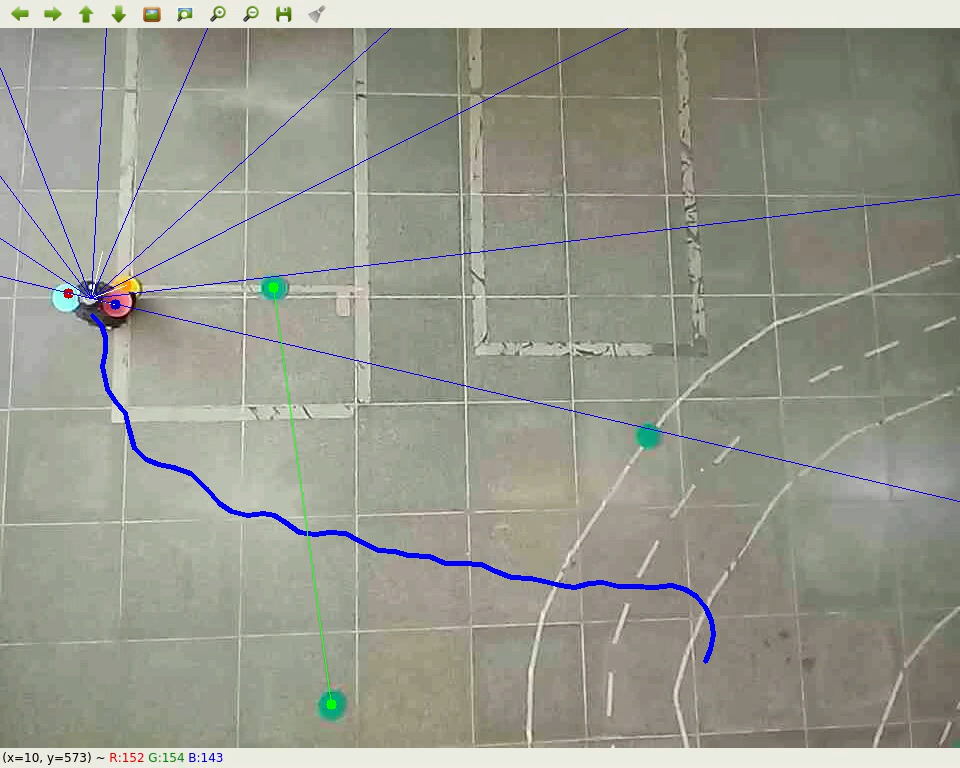
\includegraphics[width=\textwidth]{images/test_env1/8.png}
    \end{subfigure}
    \caption{Images sequence of the experiment on the Turtlebot3 in the first real environment.}\label{fig:frames_env1}
\end{figure}

For the final test of the network, it was used the second real environment.
In the graph, shown in Fig. \ref{fig:env2_graph}, the robot starts at the point $(0, 0)$ and even with obstacle the network was capable to arrive to the target. In Fig. \ref{fig:frames_env2} is shown by frames the trajectory made by the robot to complete the task. %So, with these results applied on real world environment we can see how effective can be a DDPG network trained in simulation environment
The robot was able to accomplish both tasks given in the real world environments.
This shows how effective can be the SAC networks, trained in a simulation environment, in completing complex tasks on physical environment.

\begin{figure}[htbp]
\centerline{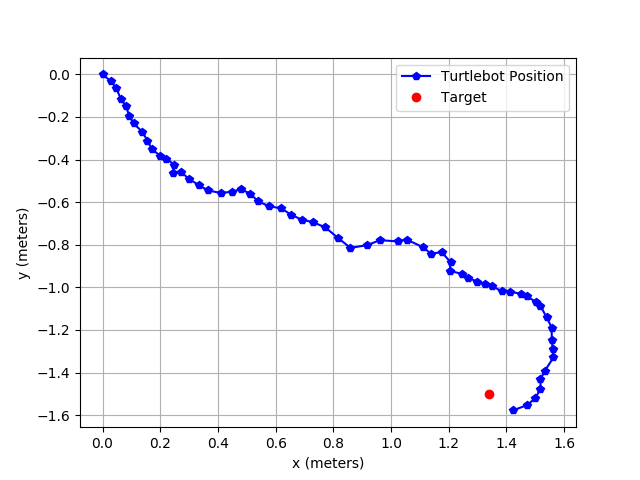
\includegraphics[width=\columnwidth]{images/test_env2.png}}
\caption{Trajectory of the Turtlebot3 in the second real environment}
\label{fig:env2_graph}
\end{figure}

\begin{figure}[htbp]
    \centering
    \begin{subfigure}[b]{0.115\textwidth}
        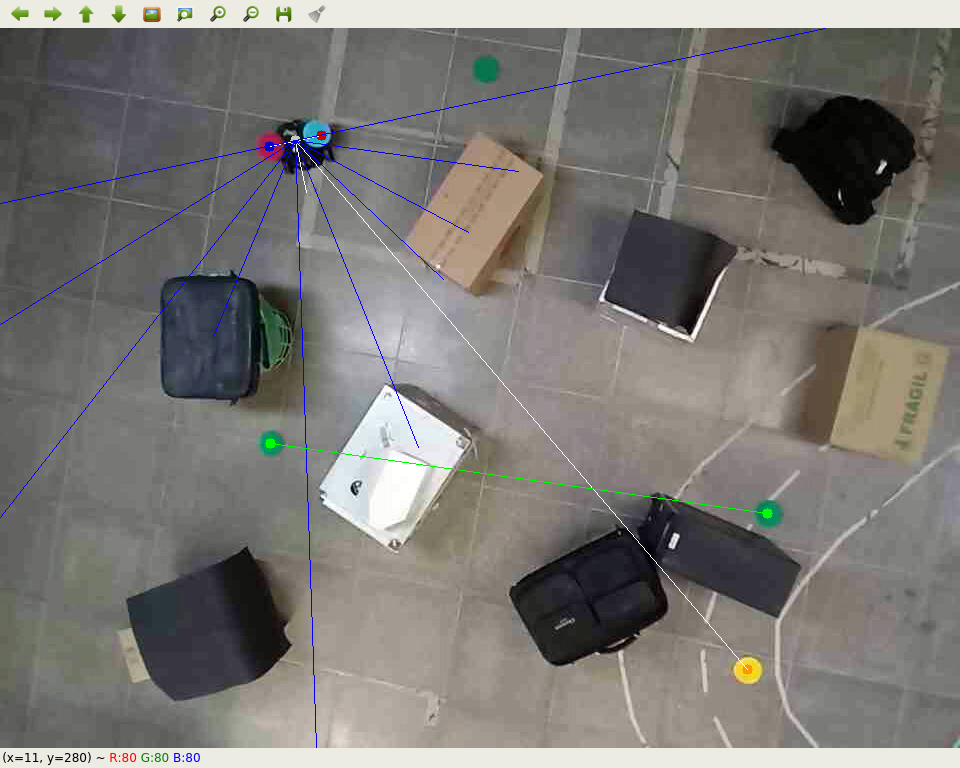
\includegraphics[width=\textwidth]{images/test_env2/1.png}
    \end{subfigure}
    \hfill
    \begin{subfigure}[b]{0.115\textwidth}
        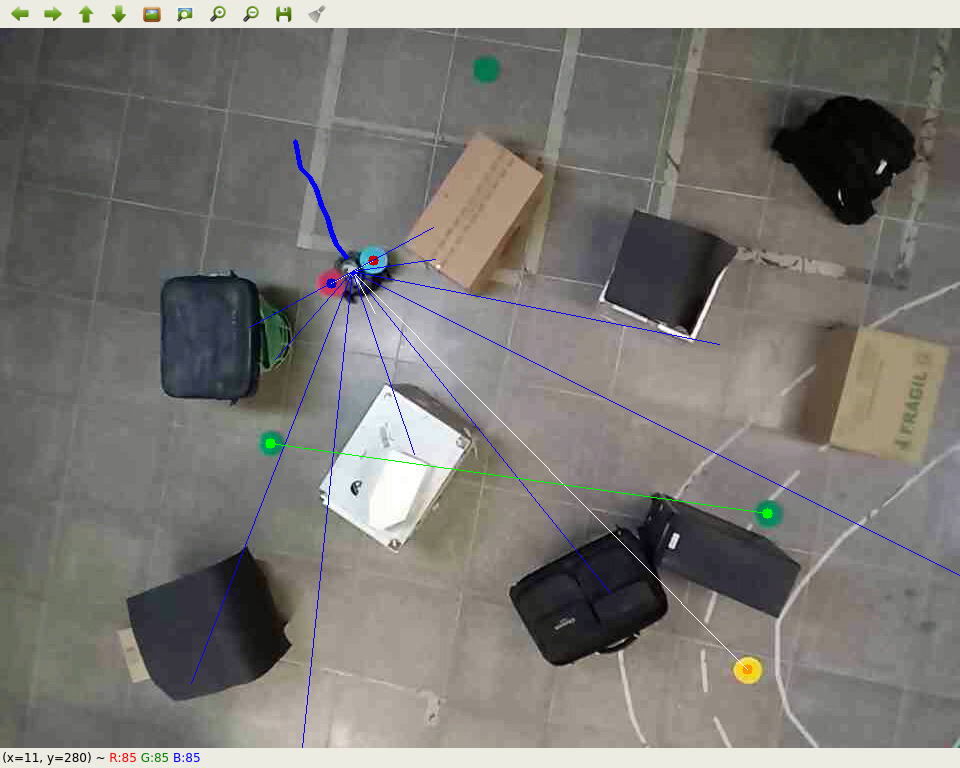
\includegraphics[width=\textwidth]{images/test_env2/2.png}
    \end{subfigure}
    \hfill
    \begin{subfigure}[b]{0.115\textwidth}
        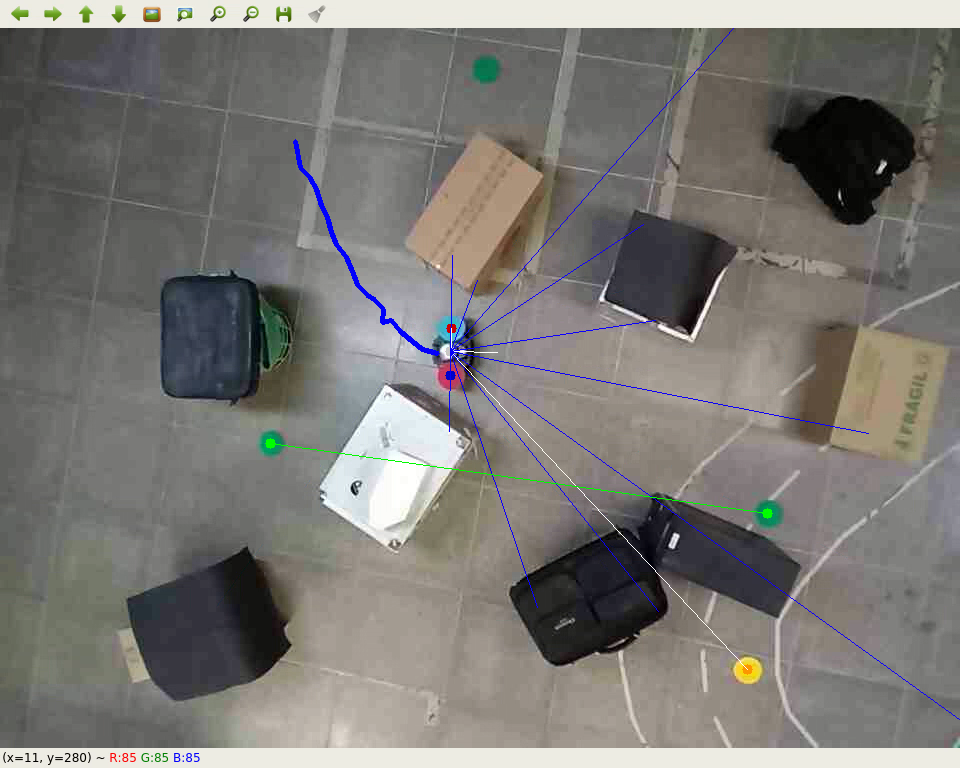
\includegraphics[width=\textwidth]{images/test_env2/3.png}
    \end{subfigure}
    \hfill
    \begin{subfigure}[b]{0.115\textwidth}
        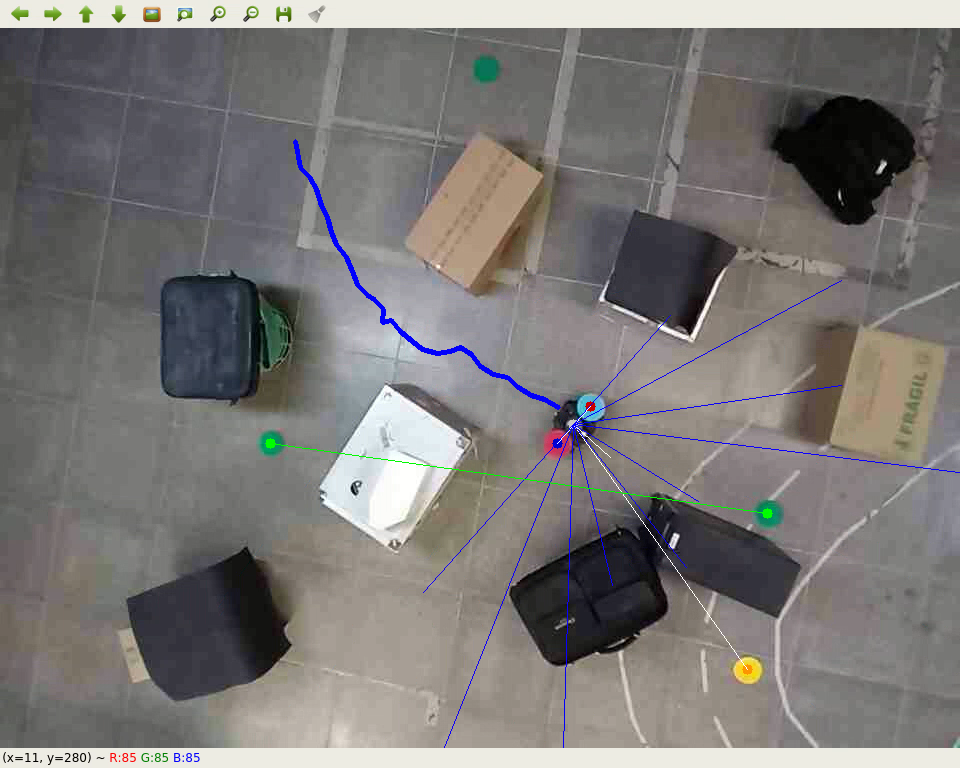
\includegraphics[width=\textwidth]{images/test_env2/4.png}
    \end{subfigure}
    \newline
    \begin{subfigure}[b]{0.115\textwidth}
        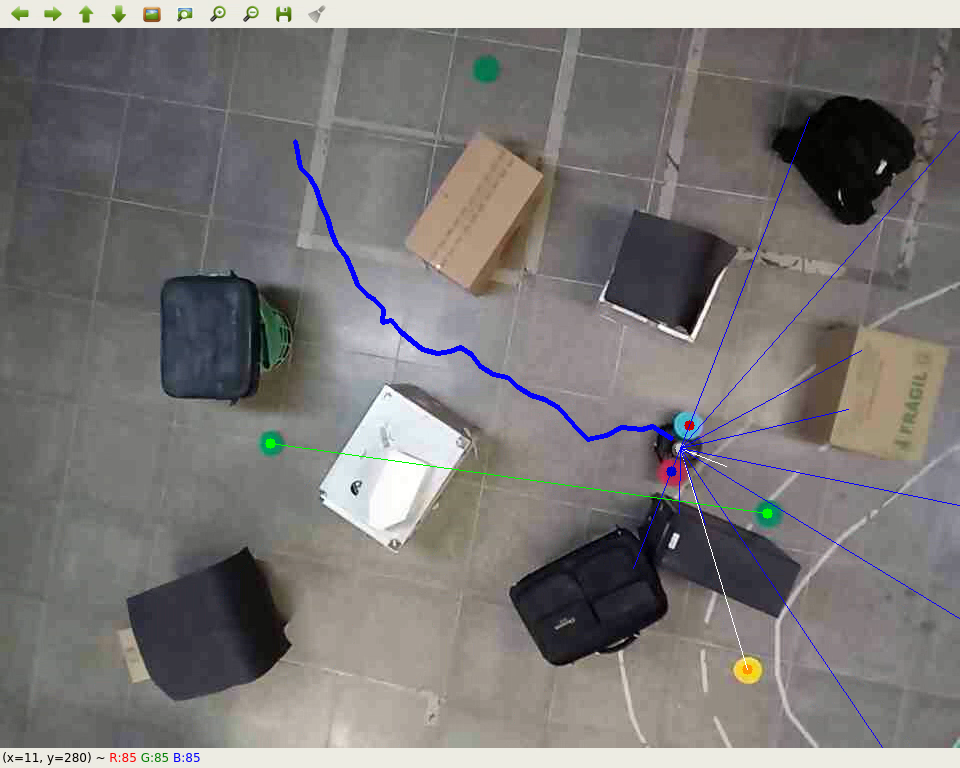
\includegraphics[width=\textwidth]{images/test_env2/5.png}
    \end{subfigure}
    \hfill
    \begin{subfigure}[b]{0.115\textwidth}
        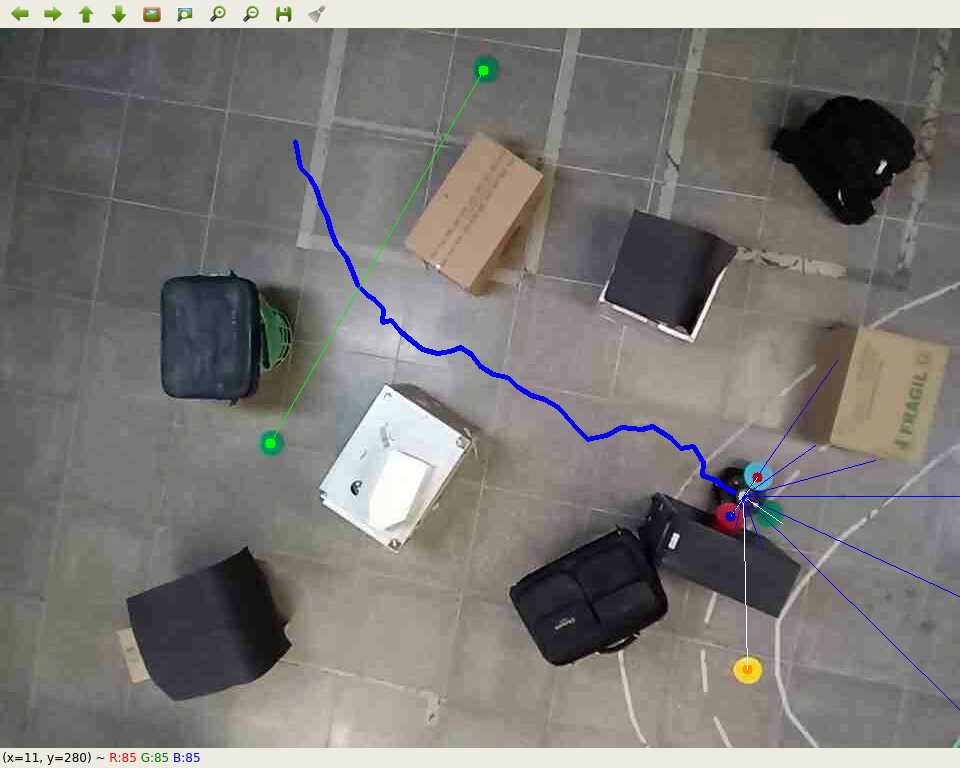
\includegraphics[width=\textwidth]{images/test_env2/6.png}
    \end{subfigure}
    \hfill
    \begin{subfigure}[b]{0.115\textwidth}
        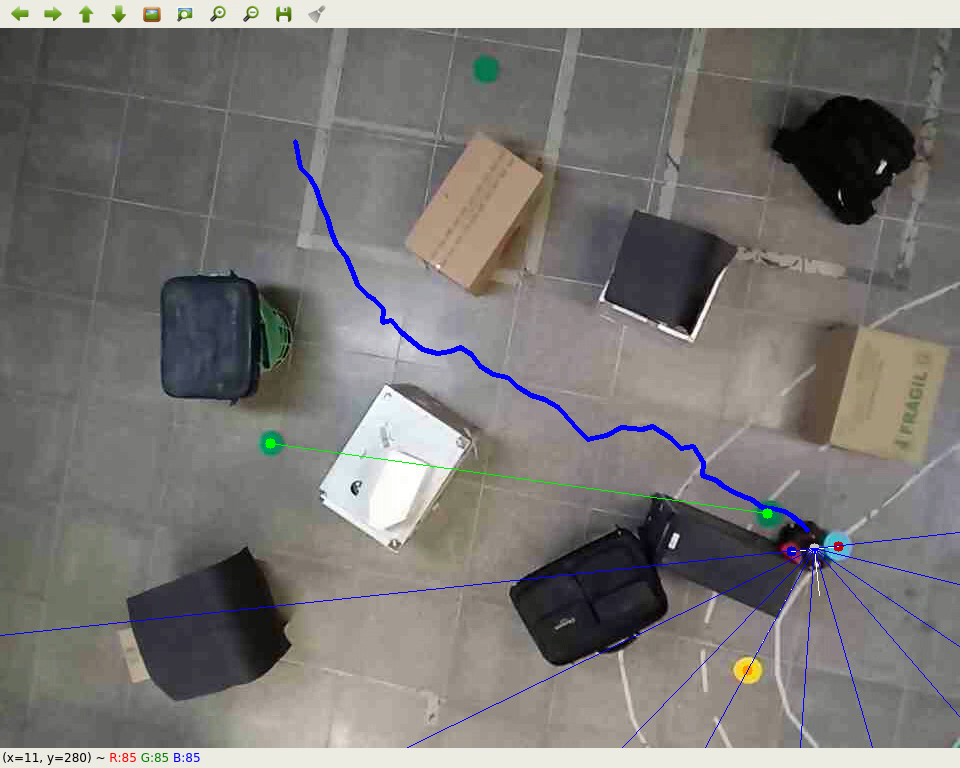
\includegraphics[width=\textwidth]{images/test_env2/7.png}
    \end{subfigure}
    \hfill
    \begin{subfigure}[b]{0.115\textwidth}
        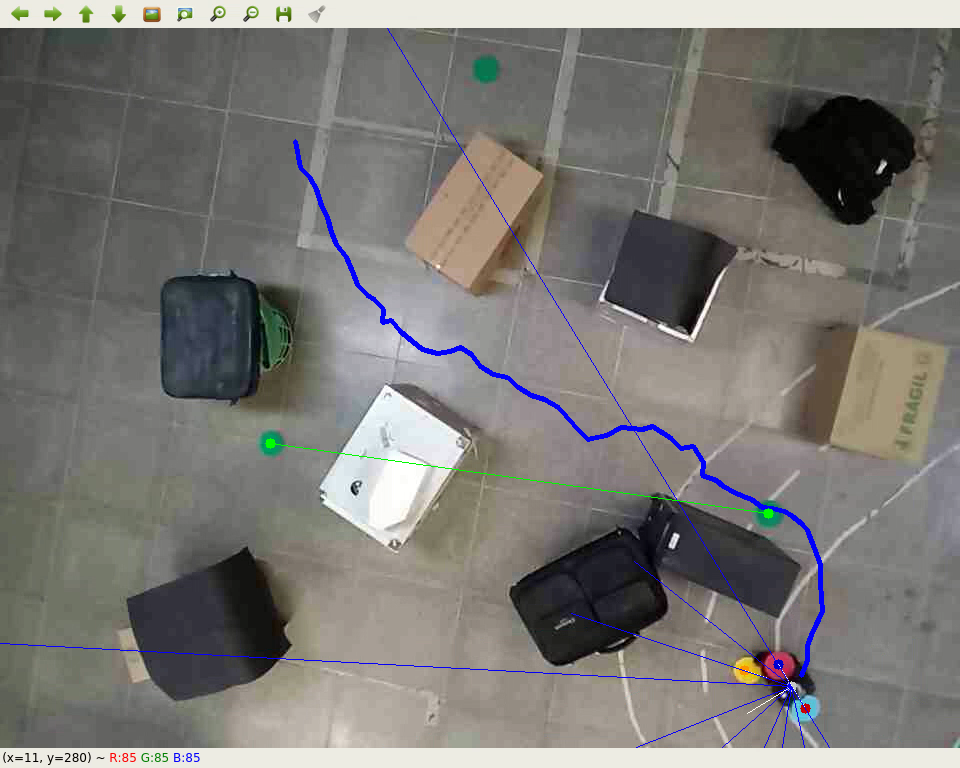
\includegraphics[width=\textwidth]{images/test_env2/8.png}
    \end{subfigure}
    \caption{Images sequence of the experiment on the Turtlebot3 in the second real environment.}\label{fig:frames_env2}
\end{figure}

\section{Conclusion}

In this paper a SAC network was used in navigation of a mobile robot through continuous control in a virtual and real environments.
Thus, a deep reinforcement learning network algorithm was able to solve the problem of robot navigation.
The experiment consisted that the robot could reach a target position in different simulated environments.
In order to accomplish this objective a reward function was proposed. The SAC network outputs were the linear and angular velocity for the robot.
%It was proposed as a task that the robot could reach a target position in different simulated environments; therefore, it was created a reward function so that the SAC network could give as results the linear and angular velocity for the robot.
%sei la tbm KKSDKK 
All the network structure created was trained on the Gazebo simulation environments before using the network in the real environments.

With the training results obtained on the simulation environments, it was analyzed the performance of the intelligent agent algorithm in the task of avoiding obstacles and getting to the final goal. 
On the two real environments proposed, the algorithm was able to complete the task of the navigation to get to a target defined on the map.
% , however, in the last environment it was observed that sometimes even after many training episodes the mobile robot would still collide with some obstacle.

It is possible to conclude that SAC networks are suitable for the development of applications that need a continuous control on the robotics.
The Deep-RL networks can produce excellent results if the reward system is well-made for the problem that it wants to solve.
It was proved that intelligent agents can move around in a complex real environments by just training in simulated environments without any previous knowledge of the scenario.
In a future work, we are planning to compare performance of the SAC and other Deep-RL strategy in the task of navigation of mobile robots.

\bibliographystyle{IEEEtran}
\bibliography{IEEEabrv,bibliography}




\end{document}
